\documentclass{article}

\usepackage[submission]{colm2026_conference}
\usepackage{microtype}
\usepackage{graphicx}
\usepackage{booktabs}
\usepackage{amsmath}
\usepackage{amssymb}
\usepackage{xcolor}
\usepackage{multirow}
\usepackage{lineno}

\usepackage{hyperref}
\definecolor{darkblue}{rgb}{0, 0, 0.5}
\hypersetup{colorlinks=true, citecolor=darkblue, linkcolor=darkblue, urlcolor=darkblue}

\usepackage{mathtools}
\usepackage{amsthm}

% Fix tight spacing between table captions and table body
\setlength{\belowcaptionskip}{6pt}

\title{Representational Commitment: \\ Hidden-State Convergence as a Signature and Lever of Agent Consistency}

\author{Anonymous Author(s)}

\begin{document}

\ifcolmsubmission
\linenumbers
\fi

\maketitle

\begin{abstract}
In production agent systems, operators need to know which inputs will produce stable behavior before committing to a trajectory. We introduce \textbf{representational commitment}: when hidden states converge across independent runs of the same input at a fixed agent step, the model has settled on a stable interpretation and downstream behavior is consistent; when they diverge, behavior scatters. On Llama-3.1-70B with ReAct on HotpotQA (100 questions $\times$ 10 runs), activation similarity at step~4 predicts behavioral consistency ($r = -0.35$; partial $r = -0.45$ after difficulty controls), with temporal specificity (absent at steps~1--2, peak at step~4) and spatial specificity (layers 32--80). The signal tracks \emph{process} consistency, not per-run correctness: committed-wrong and committed-correct questions are representationally indistinguishable, revealing commitment as a confidence axis orthogonal to accuracy. The phenomenon replicates across three model families (Llama~70B, Qwen~72B, Phi-3~14B) and two benchmarks (StrategyQA: $r = -0.83$). Commitment is both detectable---a runtime monitor achieves AUROC~0.97---and inducible: a prompting intervention raises convergence ($d = 0.97$) and cuts behavioral variance by 28\% ($d = 0.33$, $p = .001$), with a bootstrap mediation analysis confirming the representational shift statistically accounts for the behavioral change ($p < .001$).
\end{abstract}

%%%%%%%%%%%%%%%%%%%%%%%%%%%%%%%%%%%%%%%%%%%%%%%%%%%%%%%%%%%%%%%%%%%%%%%%%%%%%%%
\section{Introduction}
%%%%%%%%%%%%%%%%%%%%%%%%%%%%%%%%%%%%%%%%%%%%%%%%%%%%%%%%%%%%%%%%%%%%%%%%%%%%%%%

LLM-based agents combine language models with tool use and multi-step reasoning \citep{react, cot}. They face a familiar reliability problem: \emph{behavioral inconsistency}. With non-zero temperature, the same system may take different actions, explore different paths, and sometimes answer differently on repeated runs. Deployments usually log one trajectory per input, so inconsistency shows up as hard-to-debug variance in production and in benchmarks.

Prior work shows that divergence concentrates at early decision points \citep{anonymous2026a} and that consistency amplifies outcomes without guaranteeing correctness \citep{anonymous2026b}. Those analyses stay at the level of actions. We ask whether consistency has a measurable signature in internal representations.

We show that it does. From Llama-3.1-70B \citep{llama3} during ReAct \citep{react} on HotpotQA \citep{hotpotqa}, cross-run \emph{activation similarity} (how similar hidden states are across runs of the same question at a fixed step) predicts downstream behavioral consistency. We call this \textbf{representational commitment}. When hidden states converge across runs despite different observations, the model has settled on a stable interpretation and behavior is consistent. When hidden states diverge, the representation still depends on the particular evidence path and behavior scatters.

Our contributions:
\begin{enumerate}
    \item \textbf{Phenomenon.} Representational commitment exists: cross-run hidden-state convergence at step~4 predicts behavioral consistency ($r = -0.35$, partial $r = -0.45$, $d = 1.01$) with temporal and spatial specificity. The signal replicates across three model families (Llama~70B, Qwen~72B, Phi-3~14B) and two benchmarks (StrategyQA: $r = -0.83$), at different peak layers, ruling out selection artifacts.
    \item \textbf{Mechanism.} Commitment is a confidence axis, not an accuracy axis: it tracks stability of interpretation regardless of whether that interpretation is correct (committed-wrong $\approx$ committed-correct in activation space). Observation overlap partially drives the signal in the naturalistic setting, but the model's \emph{processing} adds information beyond document identity (partial $r = -0.31$ controlling for Jaccard; $r = -0.47$ within high-overlap questions).
    \item \textbf{Application.} Commitment is both detectable and inducible. A runtime monitor achieves AUROC~0.97 from step-4 hidden states. A prompting intervention raises convergence ($d = 0.97$) and cuts behavioral variance by 28\% ($d = 0.33$, $p = .001$); mediation analysis confirms the representational shift accounts for the behavioral change ($p < .001$).
\end{enumerate}

%%%%%%%%%%%%%%%%%%%%%%%%%%%%%%%%%%%%%%%%%%%%%%%%%%%%%%%%%%%%%%%%%%%%%%%%%%%%%%%
\section{Related Work}
%%%%%%%%%%%%%%%%%%%%%%%%%%%%%%%%%%%%%%%%%%%%%%%%%%%%%%%%%%%%%%%%%%%%%%%%%%%%%%%

\textbf{Behavioral consistency in agents.} \citet{anonymous2026a} introduced multi-run behavioral consistency as an agent reliability metric on HotpotQA, finding a 32--55 percentage point accuracy gap between consistent and inconsistent runs. \citet{anonymous2026b} extended this to SWE-bench, revealing that consistency amplifies outcomes rather than guaranteeing correctness. Self-consistency \citep{wang2023selfconsistency} leverages output-level variance via majority voting but does not examine internal representations.

\textbf{Probing LLM representations.} Hidden states encode truth \citep{burns2023discovering, marks2024geometry}, model confidence \citep{kadavath2022language}, and answer correctness in reasoning models \citep{stickland2024reasoning}. \citet{gnosis} showed that lightweight probes can detect incorrect generations from hidden states in single-turn settings. We extend probing to \emph{multi-step agentic settings} and find it predicts consistency but, notably, not per-run correctness.

\textbf{Representation engineering.} \citet{zou2023repe} introduced representation reading and control; \citet{turner2023steering} demonstrated activation steering for behavioral modification. \citet{anthropic_persona} extracted ``persona vectors'' encoding character traits, and \citet{anthropic_axis} identified an ``assistant axis'' governing default model behavior. Our work identifies another candidate axis in activation space: \emph{commitment}, the degree to which multi-run trajectories collapse to similar internal states.

%%%%%%%%%%%%%%%%%%%%%%%%%%%%%%%%%%%%%%%%%%%%%%%%%%%%%%%%%%%%%%%%%%%%%%%%%%%%%%%
\section{Method}
%%%%%%%%%%%%%%%%%%%%%%%%%%%%%%%%%%%%%%%%%%%%%%%%%%%%%%%%%%%%%%%%%%%%%%%%%%%%%%%

\textbf{Agent and task.} We deploy Llama-3.1-70B-Instruct \citep{llama3} in a ReAct \citep{react} agent on HotpotQA \citep{hotpotqa}. The agent iterates Thought $\rightarrow$ Action $\rightarrow$ Observation using Search, Retrieve, and Finish tools. We select 100 questions from the validation set: 50 ``easy'' (comparison questions with yes/no answers) and 50 ``hard'' (multi-hop requiring 2+ retrieval steps). Each question is run 10 times with temperature $T{=}0.5$\footnote{We chose $T{=}0.5$ as a moderate setting that produces meaningful behavioral variance; $T{=}0$ would yield identical runs (trivial consistency) and $T{=}1.0$ introduces excessive noise. Temperature sensitivity is a natural extension.} and maximum 25 steps, yielding 988 total trajectories.\footnote{12 runs excluded due to incomplete hidden state extraction.} At step~4 (the primary analysis step), 99 of 100 questions have sufficient data; one question's runs all terminated by step~3.

\textbf{Hidden state extraction.} The model runs on 8$\times$80GB GPUs with pipeline parallelism (10 layers per GPU). At every agent step, we extract the hidden state at the last token position from layers $\ell \in \{0, 8, 16, \ldots, 80\}$, producing $\mathbf{h}_{\ell}^{(s)} \in \mathbb{R}^{8192}$ per step $s$ and layer $\ell$.

\textbf{Behavioral consistency.} We measure two complementary metrics across the 10 runs of each question: (1)~the coefficient of variation (CV) of step counts, capturing trajectory-length consistency, and (2)~action sequence diversity, defined as the proportion of unique action sequences among runs, capturing trajectory-structure consistency. Lower values on both indicate more consistent behavior.

\textbf{Activation similarity.} For each question $q$ at step $s$ and layer $\ell$, we compute the mean pairwise cosine similarity across runs:
\begin{equation}
\text{Sim}_q^{(s,\ell)} = \binom{n}{2}^{-1} \sum_{i < j} \cos\!\left(\mathbf{h}_{\ell,i}^{(s)},\; \mathbf{h}_{\ell,j}^{(s)}\right)
\end{equation}
where $n$ is the number of runs with hidden states at step $s$. We examine the Pearson correlation between $\text{Sim}_q^{(s,\ell)}$ and $\text{CV}_q$ across all questions. At $n{=}100$ questions, this design has 80\% power to detect $|r| \geq 0.28$ (two-tailed $\alpha = 0.05$); the observed $r = -0.35$ is comfortably above this threshold. Cross-model replication on three independent 100-question samples ($3 \times 100 = 300$ question-level observations) provides effective replication.

%%%%%%%%%%%%%%%%%%%%%%%%%%%%%%%%%%%%%%%%%%%%%%%%%%%%%%%%%%%%%%%%%%%%%%%%%%%%%%%
\section{Results}
%%%%%%%%%%%%%%%%%%%%%%%%%%%%%%%%%%%%%%%%%%%%%%%%%%%%%%%%%%%%%%%%%%%%%%%%%%%%%%%

We first link activation similarity to behavioral consistency on Llama~70B (\S\ref{sec:res-sim}). \S\ref{sec:temporal}--\ref{sec:boundaries} cover timing, difficulty, shallow baselines, and limits of the signal. \S\ref{sec:crossmodel} and \S\ref{sec:strategyqa} replicate across models and benchmarks. \S\ref{sec:runtime} and \S\ref{sec:intervention} give a runtime predictor and the prompting experiment.

\subsection{Activation Similarity Predicts Consistency}
\label{sec:res-sim}

Figure~\ref{fig:heatmap} shows the correlation between activation similarity and behavioral CV across all step--layer combinations. A negative correlation emerges at step~4 across layers 32--80, peaking at layer~40 ($r = -0.348$, 95\% CI $[-0.48, -0.17]$, $p = 0.0006$). A 10{,}000-iteration permutation test confirms significance at all seven sampled layers from 32 to 80 (all permutation $p < 0.002$; full results in Table~\ref{tab:permutation}, Appendix~\ref{app:permutation}). The step~4 / layer~40 peak survives Bonferroni correction over all 66 step$\times$layer cells (corrected threshold $\alpha = 0.0008$; permutation $p = 0.0003$), and the same pattern replicates independently across three models at different peak layers (Llama L40, Qwen L64, Phi-3 L16; Section~\ref{sec:crossmodel}), ruling out step/layer-specific selection artifacts.

\begin{figure}[t]
\centering
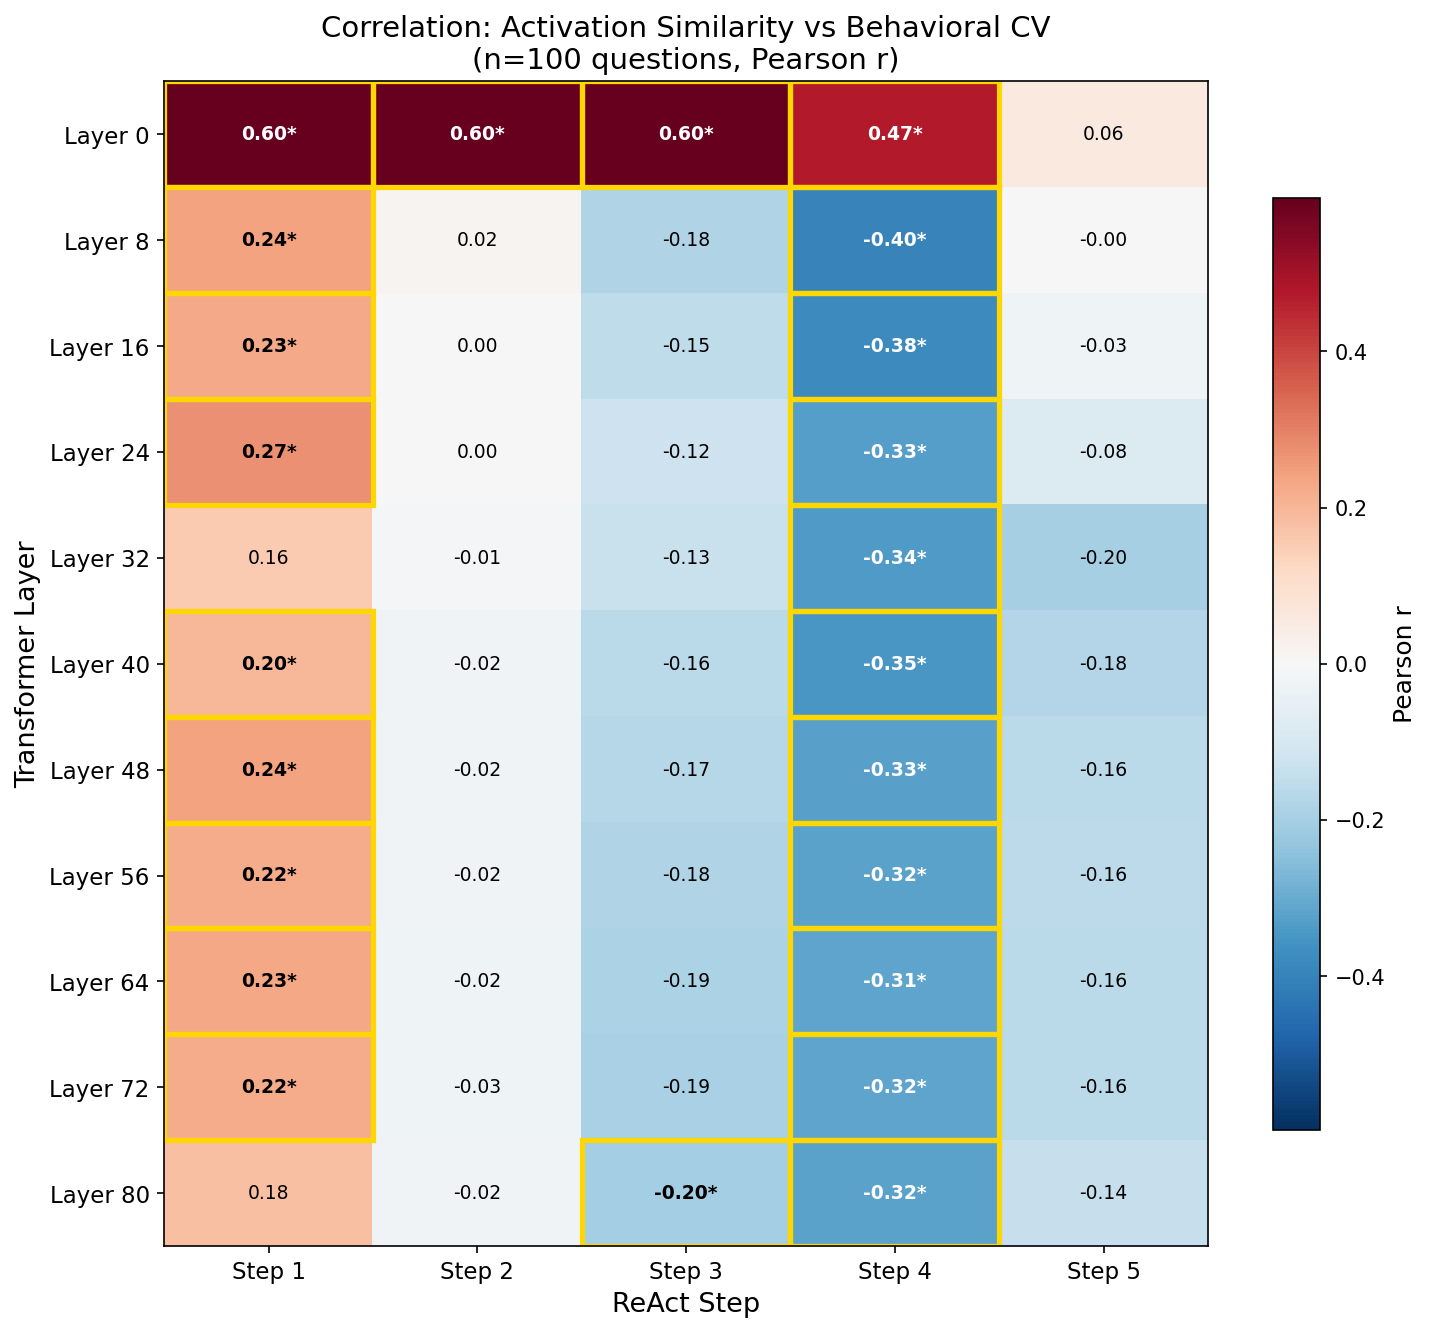
\includegraphics[width=\columnwidth]{figures/step_layer_heatmap_100q.png}
\caption{Pearson $r$ between activation similarity and behavioral CV across steps and layers ($n = 99$; one question excluded at step~4 as all runs terminated before this step). Gold borders indicate $p < 0.05$. The signal concentrates at step~4 across layers 32--80.}
\label{fig:heatmap}
\end{figure}

\textbf{Why does high similarity predict consistency?} By step~4, each run has received different observations (search results, retrieved documents). If hidden states nonetheless \emph{converge} across runs (high similarity), the model has reached a stable interpretation despite the path; we treat that as commitment, and behavior from that state is consistent. If hidden states \emph{diverge} (low similarity), the representation still tracks the particular observations in each run, so the model remains uncommitted and downstream behavior scatters.

\subsection{Temporal Profile}
\label{sec:temporal}

Figure~\ref{fig:step_progression} shows the correlation at layer~40 across steps. The signal is absent at steps 1--2, strengthens at step~3, peaks at step~4 ($r = -0.348$), and weakens at step~5. This trajectory aligns with \citet{anonymous2026a}, who found that 69\% of behavioral divergence begins at step~2. The representational commitment signal appears two steps later, capturing the model's response to the accumulated evidence.

\begin{figure}[t]
\centering
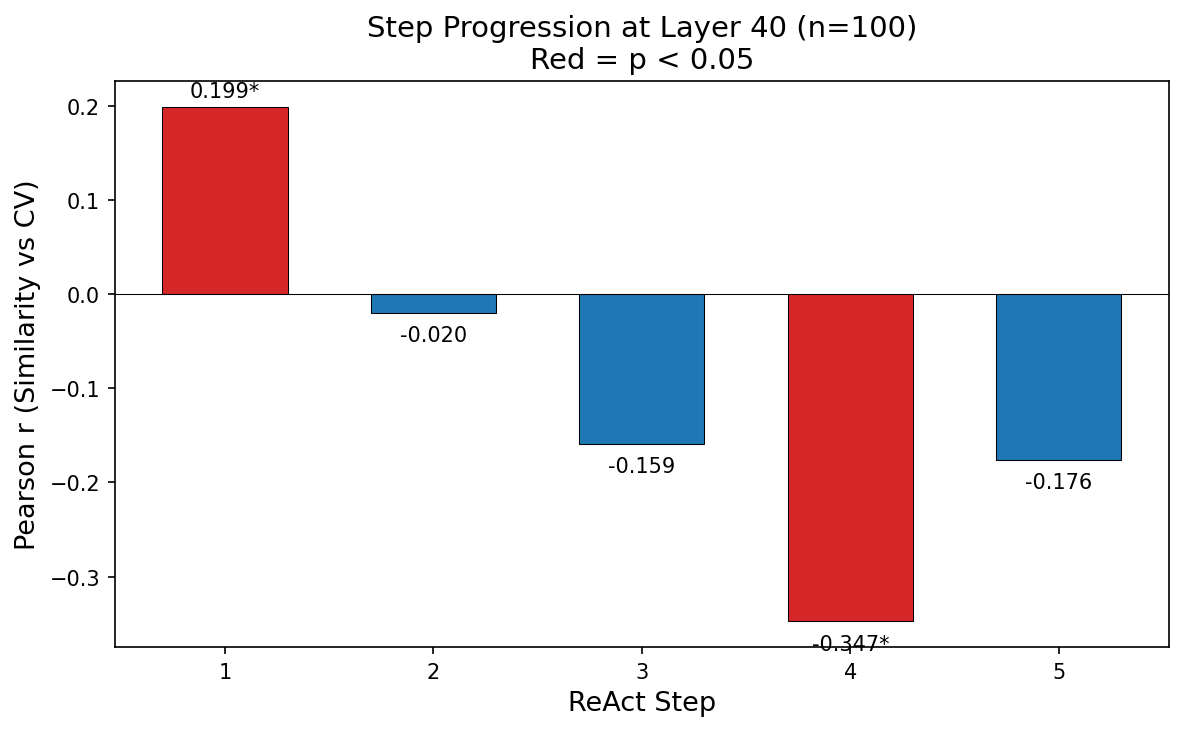
\includegraphics[width=\columnwidth]{figures/step_progression_layer40_100q.png}
\caption{Correlation between activation similarity and CV at layer~40 across steps. The consistency signal peaks at step~4.}
\label{fig:step_progression}
\end{figure}

\subsection{Controlling for Task Difficulty}

Both activation similarity and CV could be driven by task difficulty. Partial correlation controlling for accuracy and difficulty label \emph{increases} the signal from $r = -0.35$ to $r = -0.45$ (95\% CI $[-0.59, -0.29]$, $p < 10^{-5}$) at layer~40, with all layers 32--80 strengthening (partial $r$: $-0.38$ to $-0.46$; Appendix~\ref{app:partial}). Difficulty was partially \emph{suppressing} the signal, confirming it reflects a genuine representational property independent of task characteristics.

\subsection{Ruling Out Simple Baselines}

We compare hidden state similarity against simpler potential predictors of consistency (full results in Table~\ref{tab:baselines_full}, Appendix~\ref{app:baselines}). Question length ($r = 0.10$, $p = .31$), context size ($r = 0.04$, $p = .66$), and thought length ($r = 0.12$, $p = .24$) do not predict CV. A multiple regression (CV $\sim$ similarity + question length + accuracy) yields $R^2 = 0.30$; similarity ($t = -4.73$, $p < 10^{-5}$) and accuracy ($t = -4.41$, $p < 10^{-4}$) are the only significant predictors.

\textbf{Observation similarity.} A natural concern is that runs retrieving similar documents will have both similar hidden states \emph{and} similar behavior, so the commitment signal could reflect shared input rather than internal processing. We measure three forms of observation overlap across runs at steps~1--3 (before the step-4 analysis point): Jaccard similarity of retrieved document sets, TF-IDF cosine similarity of concatenated observation text, and search-query overlap ($n = 94$ questions with complete data). Observation similarity does predict CV: TF-IDF $r = -0.63$ ($p < 10^{-5}$), Jaccard $r = -0.40$ ($p < 10^{-4}$). Moreover, activation similarity and TF-IDF observation similarity are correlated ($r = 0.69$), as expected since hidden states are computed from the full context including observations.

Critically, however, activation similarity survives control for \emph{document identity}: partial $r = -0.31$ ($p = .003$) after controlling for Jaccard similarity, accuracy, and difficulty (VIF $< 2$ for all predictors). This means the commitment signal captures information about the model's processing that goes beyond which documents were retrieved. Full-text TF-IDF control absorbs the signal (partial $r = 0.09$, n.s.), but this is expected: TF-IDF encodes the \emph{content} of observations, which is part of the model's input and thus mechanically determines hidden states. The relevant test is whether the model's \emph{representation} adds information beyond document identity, and it does.

A within-group analysis sharpens the point: among questions where observation overlap is already very high (top quartile by TF-IDF, where runs retrieve nearly identical documents), activation similarity still predicts CV ($r = -0.47$, $p = .011$, $n = 28$). Even when the input evidence is matched, differences in how the model processes that evidence predict behavioral consistency. The intervention experiment (Section~\ref{sec:intervention}) provides the strongest evidence: changing only the step-3 prompt---not the observations---shifts hidden-state convergence ($d = 0.97$) and behavioral CV (28\% reduction), directly demonstrating that representational commitment is not merely an echo of observation overlap.

\subsection{Boundaries of the Signal}
\label{sec:boundaries}

\textbf{Per-run correctness.} Linear probes fail to predict per-run correctness from hidden states (AUC 0.34--0.56 across all configurations including single-turn generation), because correctness is primarily question-determined (64 questions are 10/10 correct, 23 are 0/10). The consistency signal is a \emph{between-run relational} property, not a within-run absolute one.

\textbf{Hard vs.\ easy questions.} The signal is driven by easy questions ($r = -0.57$, $p < 10^{-5}$) rather than hard ($r = -0.02$, $p = 0.88$). This null is \emph{predicted} by the commitment framework: if representational commitment encodes the model's confidence in its current interpretation—orthogonal to whether that interpretation is correct—then committed-wrong questions should be representationally indistinguishable from committed-correct ones, and the linear relationship between similarity and CV should collapse within hard questions where committed-wrong states dominate.

We test this directly. Among hard questions, we identify three commitment categories: \emph{committed-correct} (accuracy $\geq 0.8$), \emph{committed-wrong} (accuracy $\leq 0.2$, CV $\leq 0.15$), and \emph{uncommitted-wrong} (accuracy $\leq 0.2$, CV $> 0.15$). As predicted, committed-wrong questions show activation similarity indistinguishable from committed-correct (Llama: $0.935$ vs.\ $0.903$, $p = 0.30$; Qwen: $0.968$ vs.\ $0.952$, $p = 0.46$). The commitment axis is a \emph{confidence} axis: the model converges on stable representations whether right or wrong, analogous to a well-calibrated classifier that can be confidently wrong. This correctness-agnostic saturation collapses the linear relationship within hard questions (Figure~\ref{fig:commitment_categories}; Appendix~\ref{app:tsne}).

\begin{figure}[t]
\centering
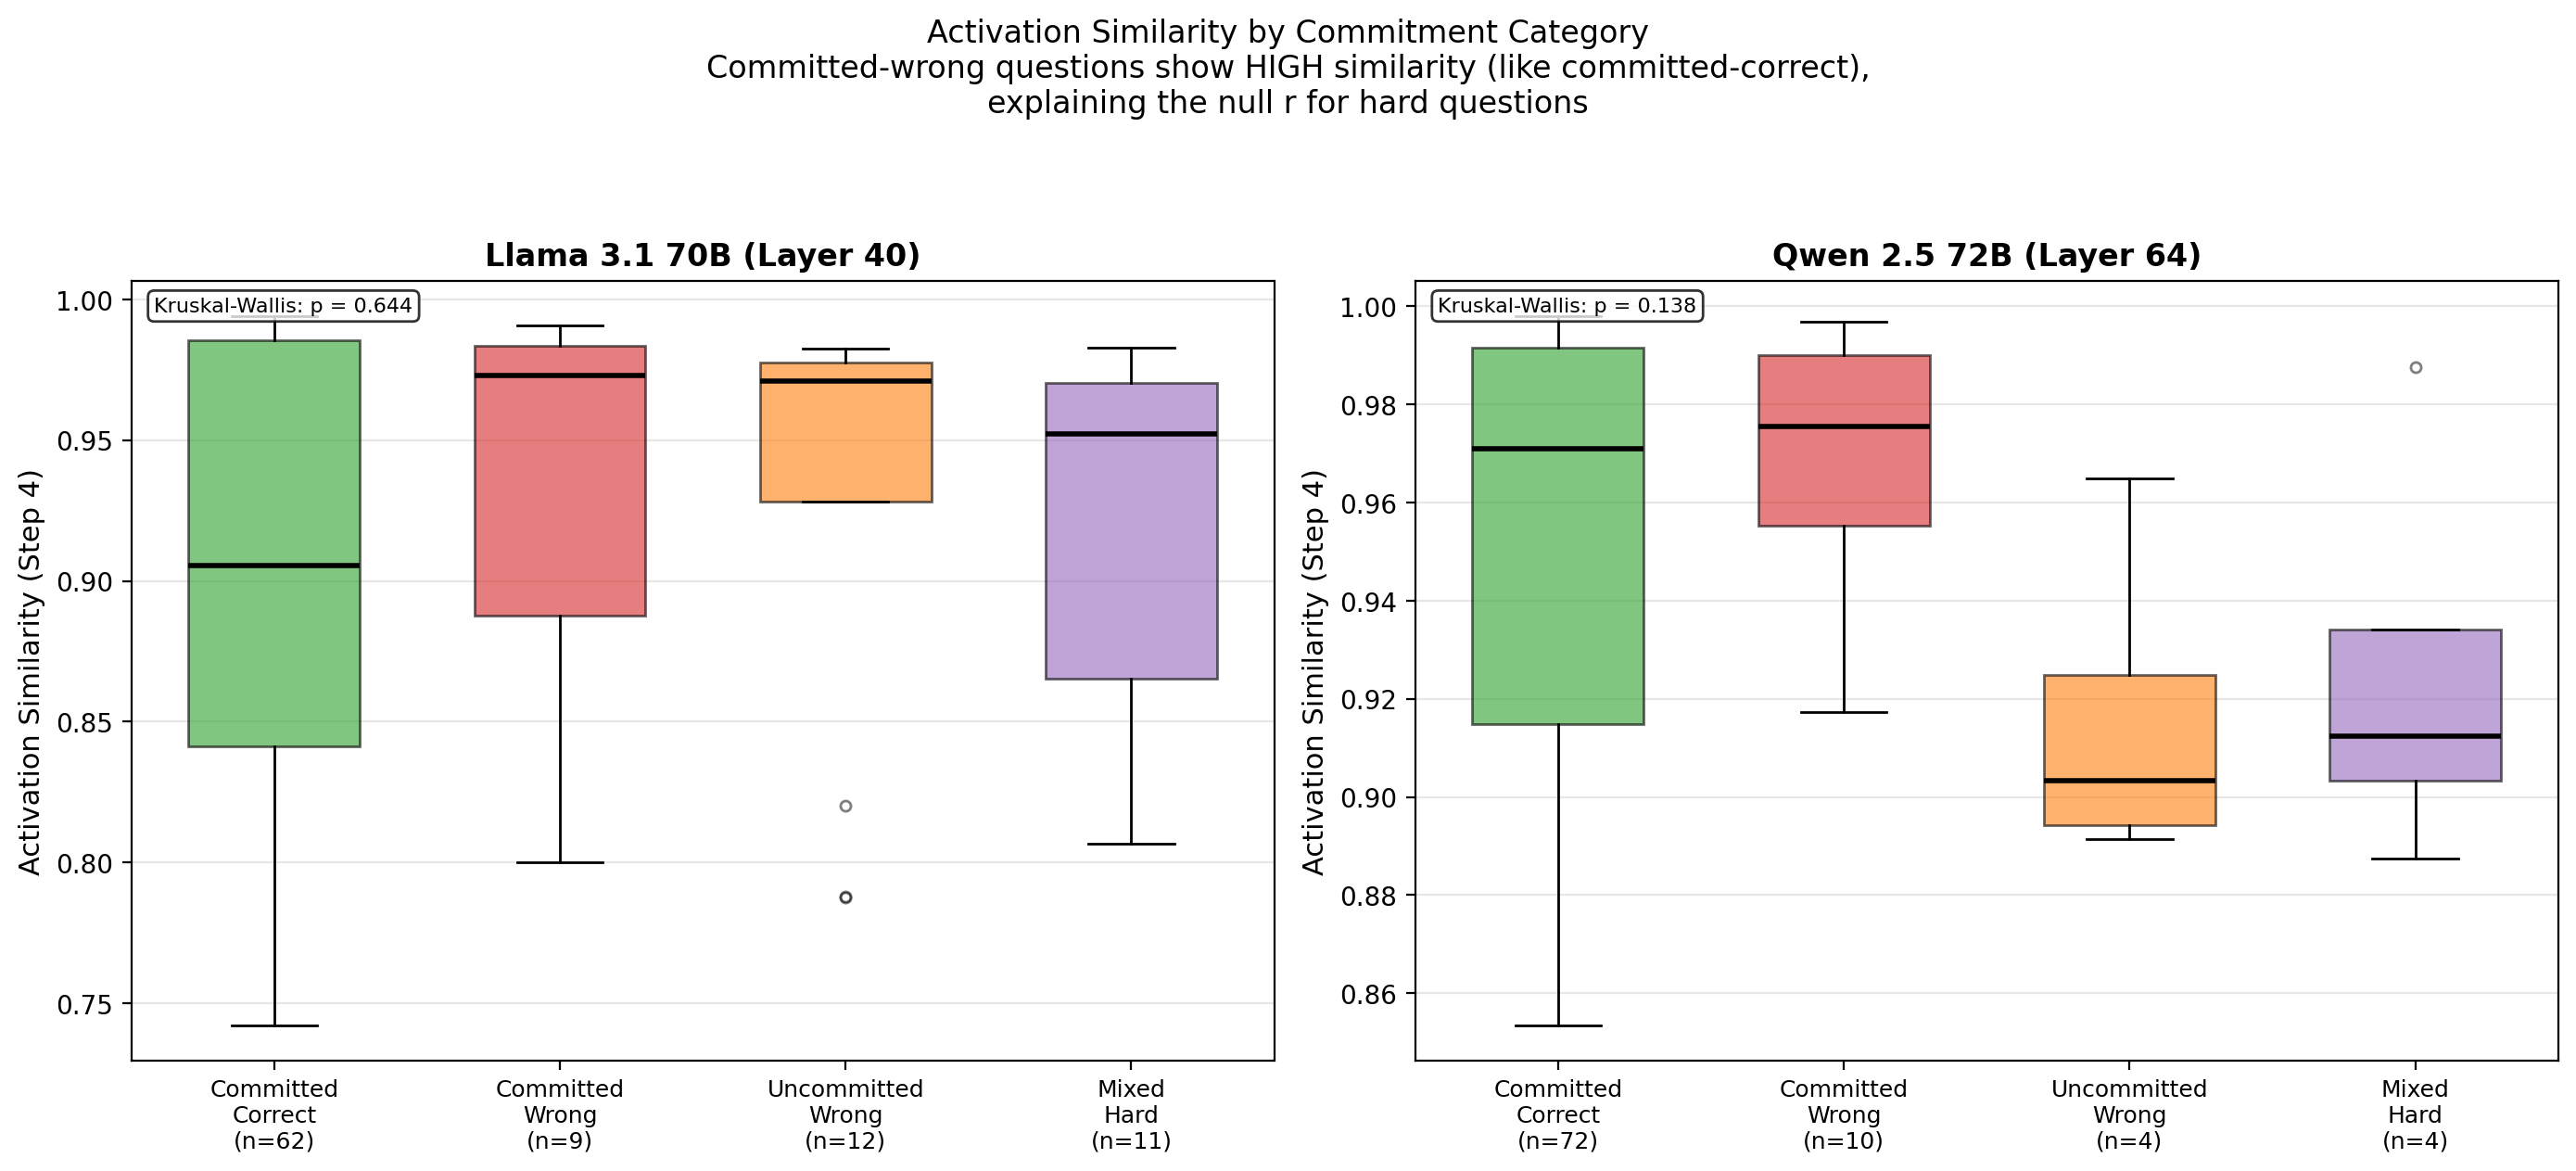
\includegraphics[width=\columnwidth]{figures/commitment_categories_boxplot.png}
\caption{Activation similarity at step~4 by commitment category. Committed-wrong questions (red) show similarity comparable to committed-correct (green), while uncommitted-wrong (orange) trend lower.}
\label{fig:commitment_categories}
\end{figure}

\textbf{Answer agreement.} Activation similarity does not predict answer agreement ($r = -0.13$, $p = 0.22$), confirming the signal reflects \emph{process} consistency (trajectory structure) rather than \emph{output} agreement.

\textbf{Prototype distance as a hard-question signal.} The preceding within-run similarity measure captures cross-run convergence \emph{within} a single question (how similar are the 10 trajectories of question $q$ to each other); we now consider a complementary \emph{between-question} measure: each question's distance from the hard-question centroid in activation space (how typical is $q$ relative to other hard questions). Although mean pairwise similarity does not predict CV among hard questions, this \emph{prototype similarity} metric does: for each hard question, we compute the cosine similarity between its mean hidden state (step~4, layer~32) and the hard-question centroid. Questions further from the centroid tend to be more consistent ($r = 0.43$, permutation $p = 0.004$, 95\% CI $[0.24, 0.63]$, Cohen's $d = 0.64$, $n{=}44$;\footnote{Six of 50 hard questions were excluded because no run produced hidden states at step~4 (all trajectories terminated in $\leq$3 steps). Excluded and included questions do not differ in accuracy ($p = .97$, Welch $t$-test) but do differ in CV ($p < .001$), as expected: short trajectories mechanically have low step-count variance regardless of behavioral consistency.} Figure~\ref{fig:prototype}). This suggests that representationally \emph{atypical} hard questions---those whose hidden states diverge from the hard-question prototype---are the ones for which the model's trajectories converge most reliably, possibly because distinctive representations anchor the reasoning path. One interpretation of the directionality: typical hard questions (close to the centroid) share surface features with many other hard questions---multiple plausible retrieval paths, ambiguous entity references, standard multi-hop structure---so the model's early evidence is compatible with several strategies, keeping trajectories spread. Atypical hard questions may have more distinctive structure that narrows the viable reasoning paths earlier, producing convergent trajectories despite the question being hard. This is consistent with the commitment framework: representational distinctiveness at step~4 may reflect the same early-settling process that within-run similarity captures, measured from a complementary angle (between-question typicality rather than within-question convergence). Variance of pairwise similarity ($r = -0.22$, $p = 0.14$), trajectory slope ($r \approx 0$), and within-run temporal stability ($r = 0.28$, $p = 0.06$) did not reach significance.

\begin{figure}[t]
\centering
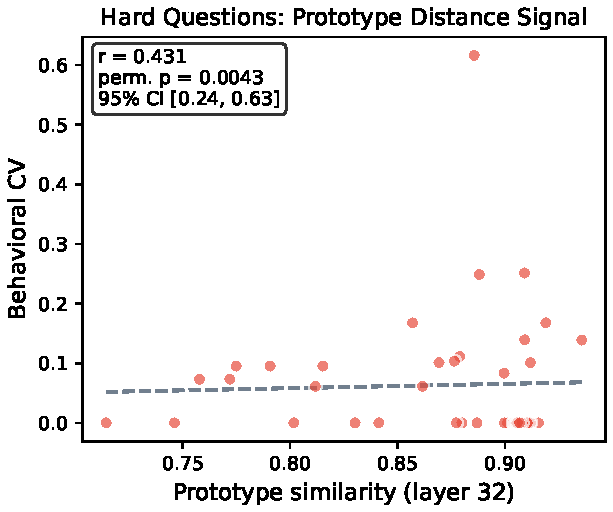
\includegraphics[width=\columnwidth]{figures/task1_prototype_signal.pdf}
\caption{Hard-question prototype signal: cosine similarity to hard-question centroid vs.\ behavioral CV (step~4, layer~32). Questions further from the centroid are more consistent ($r = 0.43$, perm.\ $p = 0.004$).}
\label{fig:prototype}
\end{figure}

\subsection{Cross-Model Validation}
\label{sec:crossmodel}

We replicate on Qwen~2.5~72B \citep{qwen2.5} (same depth/dimension as Llama, different architecture and training) and Phi-3-Medium-14B \citep{phi3} (40 layers, $d{=}5120$), running all 100 questions $\times$ 10 trials per model (988 Llama, 998 Qwen, 1{,}000 Phi-3 trajectories).

The negative correlation replicates in both. Qwen shows a stronger peak ($r = -0.65$ at layer~64, 95\% CI $[-0.74, -0.55]$, $p < 10^{-6}$). Phi-3 replicates at step~4 ($r = -0.36$ at layer~16, 95\% CI $[-0.52, -0.17]$, $p = 0.0005$, $n{=}91$) with a stronger signal at step~5 ($r = -0.58$, $p < 10^{-6}$). The later Phi-3 peak may reflect the smaller model needing one more step of evidence before committing. All sampled layers 4--36 are significant at step~4 (all $p < 0.04$; full results in Table~\ref{tab:crossmodel_full}, Appendix~\ref{app:crossmodel}).\footnote{The positive correlation at layer~0 ($r = +0.47$ for Llama, $+0.49$ for Qwen; Table~\ref{tab:crossmodel_full}) reflects input-level similarity: at the embedding layer, hidden states are determined by the (identical) input tokens, so higher similarity indexes shorter, simpler questions that also tend to be more consistent. Phi-3 lacks this pattern ($r = -0.05$, $p = .63$), likely due to its different tokenizer.}

\begin{figure}[t]
\centering
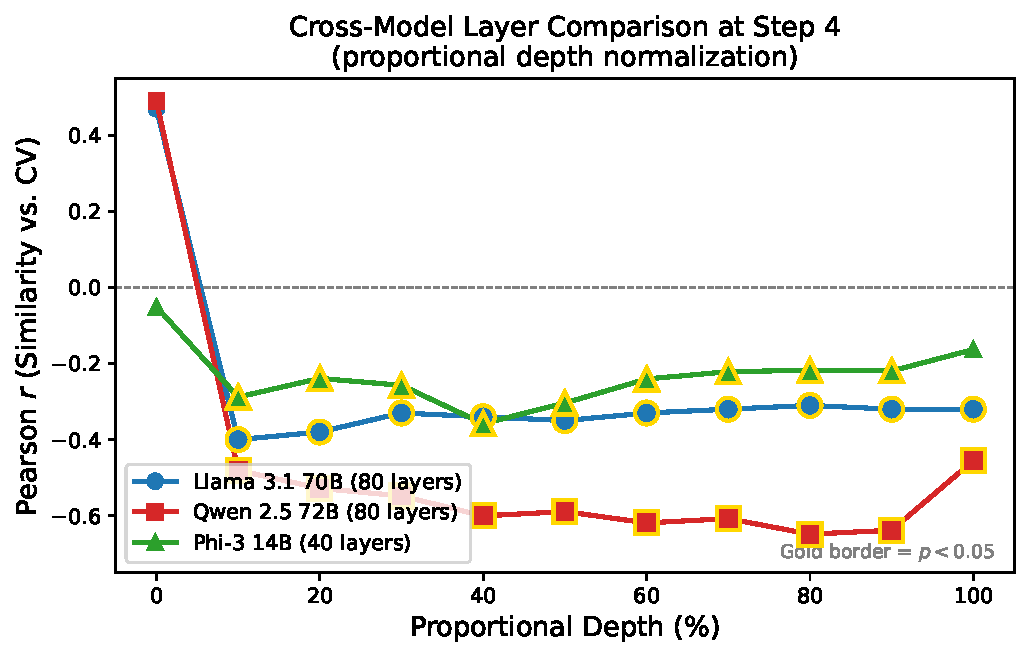
\includegraphics[width=\columnwidth]{figures/cross_model_proportional_depth.pdf}
\caption{Layer-wise correlation between activation similarity and behavioral CV at step~4 for all three models, with layers normalized to proportional depth (layer / max layer $\times$ 100\%) to enable comparison across architectures. All three models show the negative correlation characteristic of representational commitment, with Qwen strongest ($r = -0.65$) and Phi-3 weakest but significant ($r = -0.36$). The positive correlation at 0\% depth (embedding layer) for Llama and Qwen reflects an input-similarity artifact absent in Phi-3 (see text). Gold borders: $p < 0.05$.}
\label{fig:crossmodel}
\end{figure}

The \emph{peak layer} differs by model (Llama: 50\% depth; Qwen: 80\%; Phi-3: 40\%), which suggests that commitment appears across architectures but its depth profile is not fixed (Figure~\ref{fig:crossmodel}; temporal profiles in Figure~\ref{fig:step_progression_multimodel}, Appendix~\ref{app:crossmodel}).

\subsection{Cross-Benchmark Generalization: StrategyQA}
\label{sec:strategyqa}

We replicate on StrategyQA \citep{strategyqa} (implicit multi-step reasoning, yes/no answers; 50 questions balanced by answer, $\geq$2 decomposition steps, 10 runs each, $T{=}0.5$). The signal replicates strongly at step~3: $r = -0.83$ (95\% CI $[-0.90, -0.76]$, $p < 10^{-13}$), spanning all layers 8--80 ($|r| > 0.72$, $p < 10^{-8}$). The one-step-earlier peak is consistent with shorter reasoning chains (mean 5.1 vs.\ ${\sim}12$ steps). Partial correlation controlling for accuracy is unchanged ($r = -0.83$). By step~4 the signal has dissipated ($r \approx 0.07$, $p > 0.7$), consistent with commitment having largely occurred earlier (full results in Appendix~\ref{app:strategyqa}).

\subsection{Consistency Prediction from Hidden States}
\label{sec:runtime}

We evaluate whether the commitment signal is strong enough for predicting behavioral consistency at inference time. We frame this as binary classification using LOOCV with logistic regression, testing five hidden-state features and four surface-level baselines under two labeling schemes: \emph{quintile} (top/bottom 20\% by CV) and \emph{median split} (full results in Table~\ref{tab:runtime_full}, Appendix~\ref{app:runtime}).

Hidden-state features achieve strong discrimination. Under quintile labeling, a per-layer similarity profile reaches AUROC = 0.97 [0.90, 1.00] on Llama, and PCA-reduced hidden states reach 0.93 [0.85, 0.99] on Qwen. Under median split, PCA features achieve 0.85 on Llama and layer-averaged similarity reaches 0.88 on Qwen. All surface-level baselines remain near chance (AUROC $\leq 0.65$), confirming the signal resides in hidden states. Figure~\ref{fig:runtime_roc} shows ROC curves.

\begin{figure}[t]
\centering
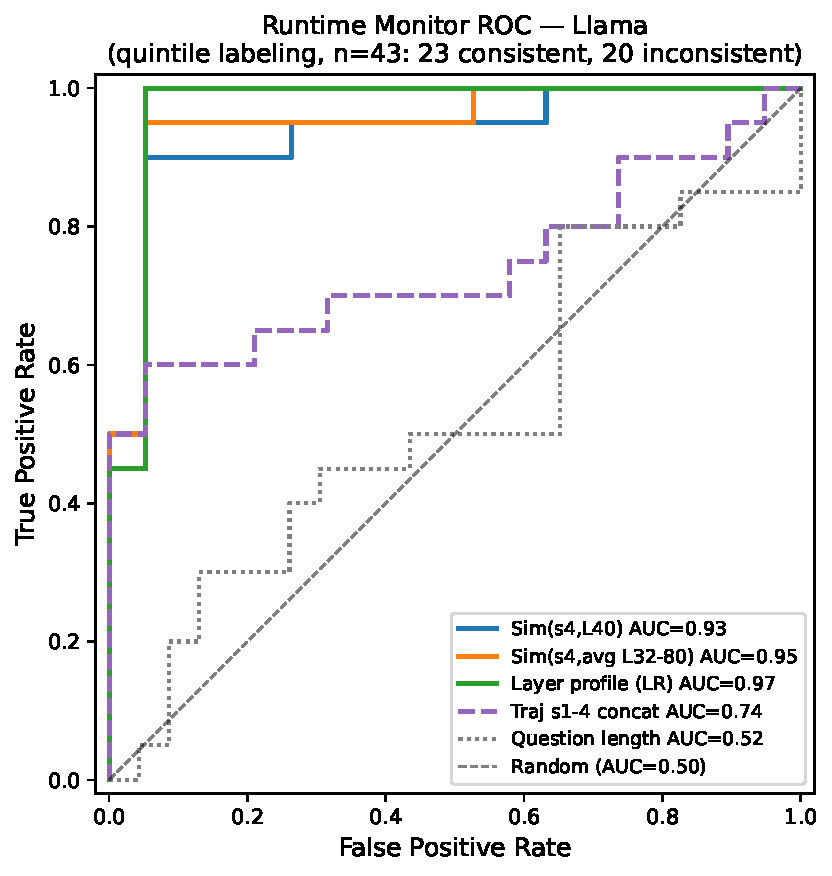
\includegraphics[width=0.48\columnwidth]{figures/runtime_monitor_roc_llama_quintile.pdf}
\hfill
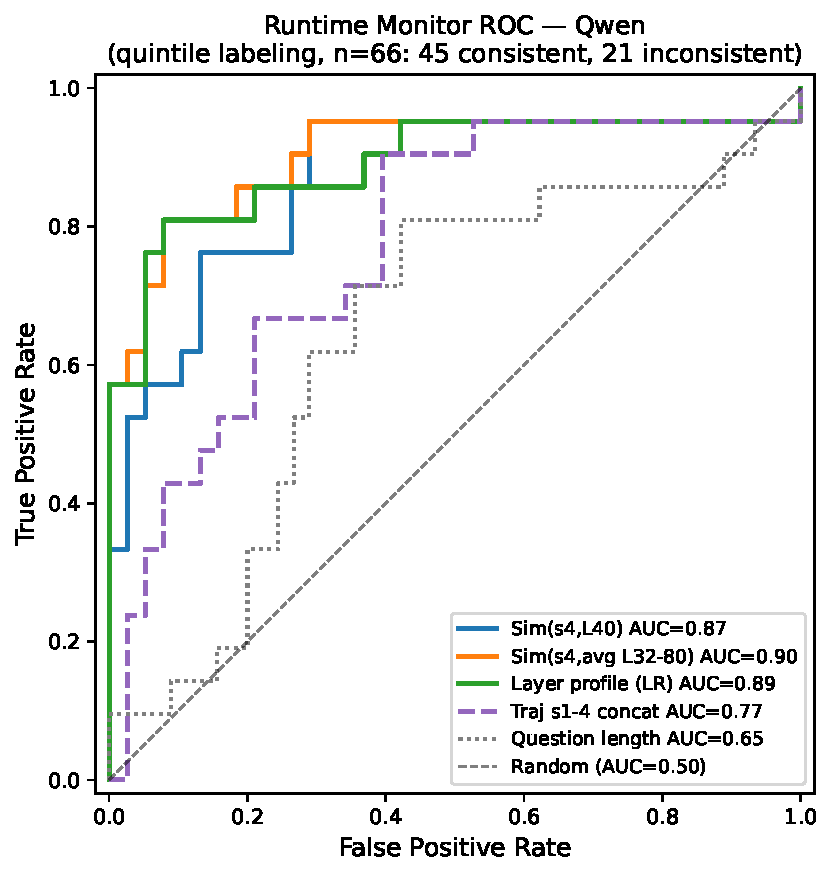
\includegraphics[width=0.48\columnwidth]{figures/runtime_monitor_roc_qwen_quintile.pdf}
\caption{ROC curves for consistency prediction (quintile labeling). Hidden-state features (solid) substantially outperform surface baselines (dashed).}
\label{fig:runtime_roc}
\end{figure}

\textbf{Practical deployment: fewer runs.} The preceding results use all 10 runs per question. In practice, a monitor must work with limited samples. We evaluate prediction quality as a function of run budget $k \in \{2, 3, 4, 5\}$ by subsampling runs (500 bootstrap iterations, LOOCV logistic regression on per-layer similarity profiles). AUROC degrades gracefully: $k{=}3$ achieves $0.81 \pm 0.07$ (95\% CI $[0.68, 0.94]$), $k{=}4$ reaches $0.87$, and $k{=}5$ reaches $0.91$, compared to the full $k{=}10$ baseline of $0.97$ (Figure~\ref{fig:auroc_k}). At $k{=}3$ with deterministic run selection, a precision-recall analysis finds an operating point with precision $= 0.81$ at recall $= 0.90$ (AUROC $= 0.89$). An early-exit simulation using 5-fold CV threshold selection shows that a monitor using $k{=}3$ runs achieves 70.2\% classification accuracy ($+20$pp over majority baseline) while saving 29\% of compute by short-circuiting questions identified as consistent.

\begin{figure}[t]
\centering
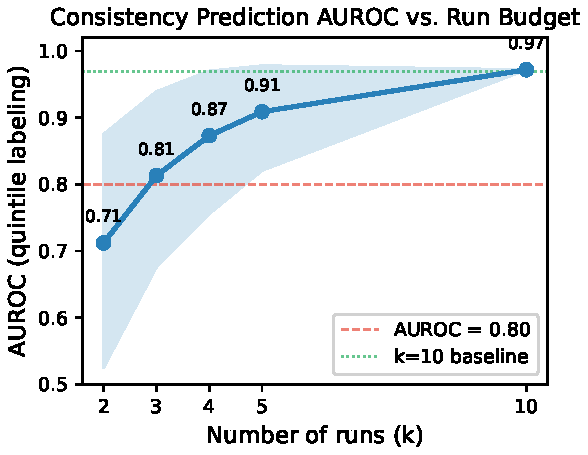
\includegraphics[width=\columnwidth]{figures/auroc_vs_k.pdf}
\caption{Consistency prediction AUROC as a function of the number of runs used to compute the hidden-state similarity features. At $k{=}3$, AUROC is $0.81 \pm 0.07$, exceeding the 0.80 threshold for practical deployment. Shaded region: 95\% bootstrap CI.}
\label{fig:auroc_k}
\end{figure}

\subsection{Intervention: Inducing Representational Commitment}
\label{sec:intervention}

If representational commitment is linked to behavioral consistency, then inducing commitment should reduce downstream variance. We test this with a prompting intervention at step~3 of the ReAct trajectory (one step before the usual commitment juncture), appending an instruction that asks the agent to commit to a reasoning strategy before continuing.\footnote{The full prompt reads: ``Based on the evidence you have gathered so far, commit to a specific reasoning strategy for solving this question. State your committed strategy clearly in your next Thought, then follow through with it. Do not change strategies or start over; build on what you have learned.''} The control condition uses the standard ReAct agent with no modification.

Because the commitment prompt adds tokens to the context window, we include a \emph{filler control}: a semantically neutral prompt of matched token length (``Please continue with the task as you normally would\ldots'') appended at the same step.\footnote{The full filler prompt reads: ``Please continue with the task as you normally would. Take the time you need to work through the problem. Consider the information you have gathered and proceed with your next step in whatever way seems most appropriate to you. There is no particular urgency; work at your own pace and follow your reasoning.''} This isolates the effect of commitment framing from mere token-count effects.

We run all three conditions on 100 HotpotQA questions (the same set used in the Qwen cross-model validation) with 10 runs per question per condition on Llama~3.1~70B ($T = 0.5$). Table~\ref{tab:intervention} reports the results. The higher accuracy relative to prior work reflects corrected matching on this 100-question subset; the original substring match on the full 200-question dataset yields 73.7\% for Llama \citep{anonymous2026a}.

\begin{table}[ht]
\centering
\caption{Three-condition prompting intervention ($n = 100$ questions, 10 runs each). The filler control matches the commitment prompt in token count but uses semantically neutral text. The critical comparison (Filler vs.\ Commitment) isolates the commitment framing effect from token-count confounds. \textsuperscript{\dag}Accuracy uses corrected matching: a response is correct if either a substring match or a token-level F1 $\geq 0.5$ holds against the gold answer, following \citet{anonymous2026a}.}
\label{tab:intervention}
\small
\begin{tabular}{lccc}
\toprule
\textbf{Metric} & \textbf{Control} & \textbf{Filler} & \textbf{Commitment} \\
\midrule
Behavioral CV & 0.112 & 0.132 & 0.095 \\
Action seq.\ diversity & 0.250 & 0.295 & 0.223 \\
Accuracy\textsuperscript{\dag} & 0.923 & 0.900 & 0.908 \\
\midrule
\multicolumn{4}{l}{\emph{Pairwise comparisons (paired $t$-test):}} \\
\midrule
 & \multicolumn{3}{c}{\textbf{Filler vs.\ Commitment} (key test)} \\
CV reduction & \multicolumn{3}{c}{28\% ($d = 0.33$, $p = .001$)} \\
Diversity reduction & \multicolumn{3}{c}{24\% ($d = 0.47$, $p < .001$)} \\
Accuracy difference & \multicolumn{3}{c}{n.s.\ ($p = .32$)} \\
\midrule
 & \multicolumn{3}{c}{\textbf{Control vs.\ Filler}} \\
CV change & \multicolumn{3}{c}{+18\% ($d = 0.18$, $p = .071$, n.s.)} \\
\midrule
 & \multicolumn{3}{c}{\textbf{Control vs.\ Commitment}} \\
CV reduction & \multicolumn{3}{c}{15\% ($d = 0.20$, $p = .044$)} \\
\bottomrule
\end{tabular}
\end{table}

The filler control does not reduce CV relative to control ($p = .071$), confirming that additional tokens alone do not improve consistency. The commitment prompt reduces CV by 28\% relative to filler (paired $t(99) = 3.29$, $p = .001$, $d = 0.33$; Wilcoxon $p < .001$), so commitment \emph{framing} accounts for the effect rather than token count alone. Action diversity shows the same pattern (24\% reduction, $d = 0.47$, $p < .001$). No condition affects accuracy (all pairwise $p > .05$; control vs.\ commitment is marginal at $p = .083$, and the filler-vs-commitment comparison, which isolates framing from token-count effects, shows no accuracy difference, $p = .32$). This pattern matches the correctness-agnostic view of commitment (Section~4.4): inducing commitment makes the model adhere more firmly to whatever interpretation it has formed (correct or incorrect), so mostly-correct items become more consistently correct and mostly-wrong items more consistently wrong, which cancels in aggregate accuracy.

\textbf{Interpreting the three pairwise comparisons.} The filler condition trends toward \emph{higher} variance than control (CV = 0.132 vs.\ 0.112, +18\%, $d = 0.18$, $p = .071$), suggesting that any prompt insertion at step~3 disrupts the natural commitment trajectory---perhaps by introducing irrelevant tokens that dilute the context signal or by being parsed as an implicit cue of uncertainty. The commitment prompt overcomes this disruption \emph{and} achieves additional tightening beyond baseline, as confirmed by the significant control-vs-commitment comparison (15\% CV reduction, $d = 0.20$, $p = .044$). Reading the three comparisons together: (i) Filler vs.\ Commitment (28\%, $d = 0.33$) isolates framing from token count; (ii) Control vs.\ Commitment (15\%, $d = 0.20$) gives the net behavioral improvement over unmodified runs; (iii) Control vs.\ Filler (+18\%, $d = 0.18$, n.s.) reveals the disruption cost of irrelevant prompt insertion. The framing effect is therefore conservative: the 28\% figure includes recovery from disruption, while the 15\% figure represents the net gain.

\textbf{Representational-level evidence.} We extracted hidden states across all three conditions and computed activation similarity at step~4 for $n{=}89$ matched questions (11 questions excluded because at least one condition had fewer than 2 runs reaching step~4 with complete hidden-state extraction; excluded questions do not differ systematically in accuracy or CV from the matched set). Figure~\ref{fig:intervention_step_progression} shows the main pattern: all three conditions produce \emph{identical} similarity trajectories through step~3 (the intervention point), then diverge sharply at step~4. The commitment condition produces the highest similarity (0.995), followed by filler (0.979) and control (0.922).

Against the filler, and holding shared prompt text fixed, the commitment framing still increases representational convergence beyond token overlap ($\Delta = +0.016$, $d = 0.97$, $p < .001$; commitment vs.\ control: $\Delta = +0.075$, $d = 1.14$, $p < .001$; all at layer~40). The filler's intermediate similarity (0.979) reflects lexical overlap from the shared prompt text: superficial convergence that does not behave like commitment, as shown by \emph{higher} behavioral variance under filler (CV = 0.132 vs.\ 0.112 for control). Only the extra convergence specific to the commitment prompt tracks lower variance. In short, the prompt changes hidden-state geometry at the commitment juncture, and that change lines up with the behavioral gains.

\textbf{Mediation analysis.} To test whether activation similarity statistically mediates the link from commitment prompting to behavioral consistency, we run a bootstrap mediation analysis (Preacher \& Hayes method, 5{,}000 iterations) on the $n{=}90$ matched filler--commitment question pairs. The indirect effect (commitment $\rightarrow$ activation similarity $\rightarrow$ CV) is significant: $ab = -0.062$, 95\% CI $[-0.094, -0.038]$, Sobel $z = -4.56$, $p < .001$. The direct effect of condition on CV, controlling for activation similarity, is not significant ($c' = +0.021$, 95\% CI $[-0.019, 0.065]$), indicating that the behavioral effect of the commitment prompt is fully accounted for by the representational shift. This is consistent with---though does not prove---a mediating pathway in which the commitment prompt reshapes hidden-state geometry, and that geometric change drives the behavioral tightening.

\begin{figure}[t]
\centering
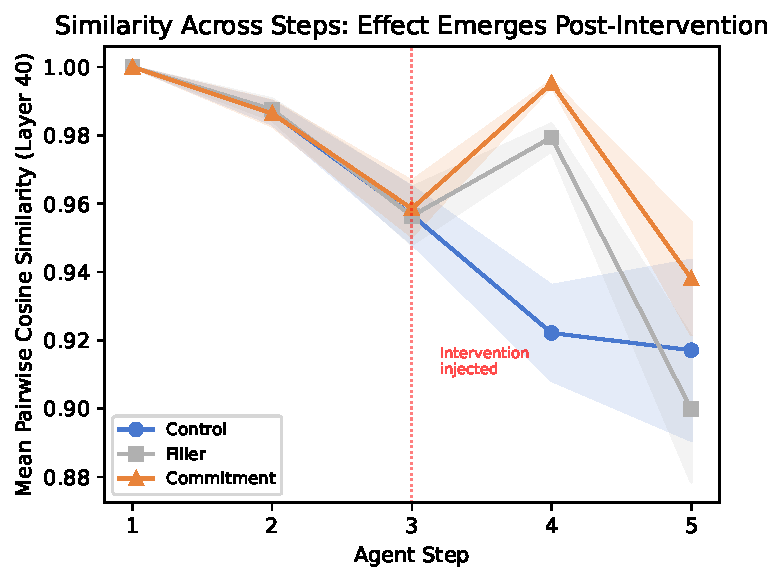
\includegraphics[width=\columnwidth]{figures/intervention_similarity_step_progression.pdf}
\caption{Activation similarity (layer~40) across agent steps for all three intervention conditions ($n{=}89$ matched questions). All conditions are identical through step~3 (intervention point, dashed line), then diverge at step~4: commitment produces the highest convergence (0.995), filler intermediate (0.979), and control lowest (0.922). There is no pre-existing gap before the intervention; divergence appears one step after, consistent with the prompt shifting geometry at the commitment juncture.}
\label{fig:intervention_step_progression}
\end{figure}

\textbf{Stratified analysis.} The effect concentrates on originally-inconsistent questions (top CV tertile, $n = 32$): filler-vs-commitment $\Delta\text{CV} = 0.069$ ($d = 0.44$, $p = .018$), while already-consistent questions show a smaller, non-significant trend ($d = 0.27$, $p = .102$), which is what we would expect if commitment mainly pulls in scattered runs.

\textbf{Question-level decomposition.} We classify each question under both conditions into consistent-correct (accuracy $\geq 0.8$), consistent-wrong (accuracy $\leq 0.2$, majority frequency $\geq 0.6$), and inconsistent, forming a 3$\times$3 transition matrix. The matrix is largely stable: 88 of 89 consistent-correct questions stay consistent-correct under commitment, all 4 consistent-wrong stay consistent-wrong, and none move from consistent-correct to consistent-wrong.\footnote{Under corrected matching, the control condition yields 89 consistent-correct, 4 consistent-wrong, and 7 inconsistent questions. The higher consistent-correct count relative to the 64 reported in Section~4.4 (which uses original substring matching) reflects questions reclassified as correct by token-F1.} The commitment intervention never degrades already-correct performance. At the question level, CV reduction and accuracy change are negatively correlated ($r = -0.32$, $p = .001$; Figure~\ref{fig:cv_acc_scatter}, Appendix~\ref{app:intervention_decomposition}): questions where commitment most reduced behavioral variance showed slight accuracy decreases, consistent with commitment amplifying whatever trajectory the model already favors (correct or not).

\textbf{Compute allocation.} We tested whether the commitment signal from $k{=}2$ initial runs could enable more efficient compute allocation by selectively retrying uncommitted questions. Using hidden states from the 53 control questions for which all 10 runs had complete step-4 hidden-state extraction (the remaining 47 had at least one run terminating before step~4 or incomplete extraction), we compared commitment-aware allocation against fixed-budget majority voting ($k_\text{init} \in \{2, 3\}$, $k_\text{extra} \in \{3, 5, 8\}$, 500 bootstrap iterations). The commitment-aware strategy does not meaningfully outperform fixed majority voting at matched compute (93.4\% vs.\ 93.1\% at ${\sim}$3 runs/question). The full $k{=}10$ signal supports strong classification (AUROC 0.97; Section~4.7), but the $k{=}2$ signal is too noisy for reliable routing. The practical payoff is mostly \emph{diagnostic}: flagging which questions will behave inconsistently, rather than directly lifting accuracy through reruns alone.

A preliminary activation steering experiment (Appendix~\ref{app:steering}) yielded mixed results: single-layer perturbation at step~4 is too late and too local, suggesting that representational commitment is a distributed process unfolding across layers and steps rather than a localized activation pattern.

\subsection{Summary of Main Findings}

Table~\ref{tab:summary} consolidates all key results across models and benchmarks.

\begin{table*}[t]
\centering
\caption{Summary statistics across all experimental conditions. Peak step and layer indicate where the activation-similarity--CV correlation is strongest. Partial $r$ controls for accuracy and difficulty. AUROC uses quintile labeling with layer-profile features. CV reduction is commitment vs.\ filler (paired).}
\label{tab:summary}
\small
\begin{tabular}{llccccccc}
\toprule
\textbf{Model} & \textbf{Benchmark} & $n$ & \textbf{Peak step} & \textbf{Peak layer (\% depth)} & \textbf{Peak $r$} & \textbf{Partial $r$} & \textbf{AUROC} & \textbf{CV red.} \\
\midrule
Llama-3.1-70B & HotpotQA   & 100 & 4 & 40 (50\%) & $-0.35$ & $-0.45$ & 0.97 & 28\% \\
Qwen-2.5-72B  & HotpotQA   & 100 & 4 & 64 (80\%) & $-0.65$ & ---     & 0.93 & --- \\
Phi-3-Medium-14B & HotpotQA & 100 & 4 & 16 (40\%) & $-0.36$ & ---     & ---  & --- \\
Llama-3.1-70B & StrategyQA  &  50 & 3 & 40 (50\%) & $-0.83$ & $-0.83$ & ---  & --- \\
\bottomrule
\end{tabular}
\end{table*}

%%%%%%%%%%%%%%%%%%%%%%%%%%%%%%%%%%%%%%%%%%%%%%%%%%%%%%%%%%%%%%%%%%%%%%%%%%%%%%%
\section{Discussion}
%%%%%%%%%%%%%%%%%%%%%%%%%%%%%%%%%%%%%%%%%%%%%%%%%%%%%%%%%%%%%%%%%%%%%%%%%%%%%%%

\textbf{Representational commitment as a new axis.} Recent work has identified linear directions encoding persona \citep{anthropic_persona}, default behavior \citep{anthropic_axis}, and truth \citep{marks2024geometry}. \emph{Commitment}, the degree to which representations converge across runs to a stable interpretation, may be another such direction. Unlike those mostly static axes, it emerges \emph{during} multi-step interaction and sharpens at a \emph{commitment juncture}. That makes it a task-state variable in agent settings: it reflects whether the model has settled into a robust internal state mid-trajectory, not a fixed property of the weights alone.

\textbf{Commitment as a linear direction.} We provide geometric evidence that commitment is well-described by a single linear direction in activation space. Defining $\mathbf{v}_{\mathrm{commit}} = \bar{\mathbf{h}}_{\mathrm{committed\text{-}correct}} - \bar{\mathbf{h}}_{\mathrm{uncommitted\text{-}wrong}}$ at layer~40 (Llama peak), we find it nearly coincides with the first principal component of the mean hidden states ($\cos = -0.98$; PC1 explains 53\% of variance). Projecting all 100 questions onto $\mathbf{v}_{\mathrm{commit}}$ yields a significant correlation with behavioral CV ($r = -0.32$, $p = 0.001$; easy: $r = -0.41$; hard: $r = -0.34$), confirming that a single direction captures much of the commitment--consistency relationship (Figure~\ref{fig:commit_proj}). The commitment direction also aligns with the easy--hard difference vector ($\cos = 0.95$), linking commitment geometry to question difficulty. In Qwen at layer~64, the projection correlation strengthens ($r = -0.59$), and a Procrustes-aligned cross-model comparison yields modest agreement ($\cos = 0.19$), though a raw PCA-space comparison shows stronger alignment ($\cos = 0.38$). The gap is interpretable: Procrustes alignment enforces a rigid rotation, asking whether the commitment axis occupies the \emph{same geometric position} in both models' activation spaces; the raw PCA comparison asks only whether both models assign large variance to a commitment-related direction, without requiring rotational equivalence. The discrepancy therefore suggests that both models develop a commitment axis---confirming universality---but this axis is architecture-specific in its orientation rather than constituting a model-invariant geometric direction, analogous to findings in cross-lingual representation alignment where similar functional structure coexists with non-isometric geometry \citep{conneau2020emerging}. Whether a universal commitment direction exists across architectures may depend on shared pretraining data or alignment procedures rather than architecture alone, and remains a question for future work.

\begin{figure}[t]
\centering
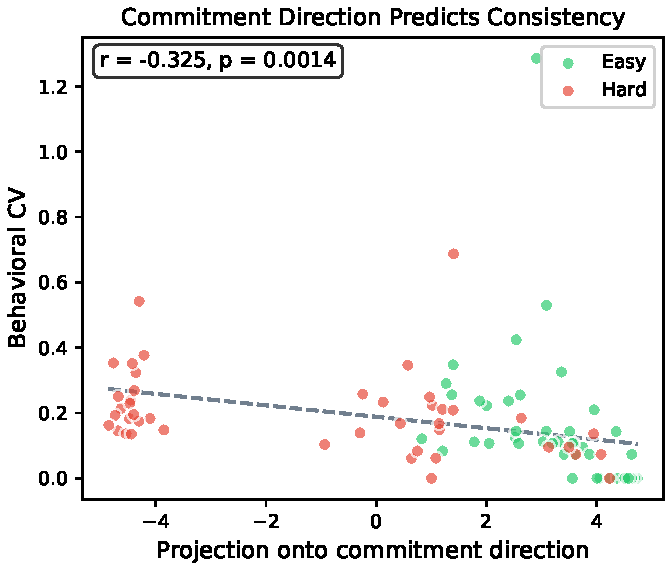
\includegraphics[width=\columnwidth]{figures/commitment_projection_scatter.pdf}
\caption{Projection of per-question mean hidden states onto the commitment direction $\mathbf{v}_{\mathrm{commit}}$ vs.\ behavioral CV. Easy questions (blue) cluster at high projection / low CV; hard questions (orange) spread across the commitment axis. Llama layer~40, step~4.}
\label{fig:commit_proj}
\end{figure}

\textbf{From measurement to reliability.} Behavioral consistency predicts downstream correctness in prior work: \citet{anonymous2026a} showed that selective prediction via unanimous agreement improves accuracy by 6--14pp at 54--62\% coverage in agentic settings, while \citet{anonymous2026b} showed that consistency amplifies outcomes in both directions. Our results supply a representational account of those behavioral patterns. The commitment signal in hidden states helps explain \emph{why} some questions yield consistent behavior and others do not. A consistency predictor (AUROC 0.97) shows the signal is visible before a trajectory finishes, which opens the door to selective prediction without running many full rollouts. The prompting experiment adds convergent evidence at both levels: the commitment prompt moves hidden-state similarity at the juncture (Section~\ref{sec:intervention}), and a bootstrap mediation analysis confirms that the representational shift statistically accounts for the behavioral change (indirect effect $p < .001$; Section~\ref{sec:intervention}).

The question-level decomposition reinforces the same story: commitment amplifies the trajectory the model is already on. We see zero transitions from consistent-correct to consistent-wrong. The practical upside is diagnostic: flag inputs where the model has not committed, then spend extra compute or review there.

\textbf{Relation to self-consistency.} Self-consistency \citep{wang2023selfconsistency} uses \emph{output} agreement to aggregate answers via majority voting. Representational commitment uses \emph{hidden-state} convergence to predict \emph{process} consistency---whether trajectories will take similar paths, not just reach similar answers. The key differences: (i)~commitment can flag inconsistency at step~4, before trajectories finish (median trajectory length ${\sim}12$ steps), enabling early intervention; (ii)~commitment predicts trajectory-structure consistency, not just final-answer agreement---indeed, activation similarity does \emph{not} predict answer agreement ($r = -0.13$, $p = .22$; Section~\ref{sec:boundaries}); (iii)~commitment requires hidden-state access, which self-consistency does not. The two approaches are complementary: self-consistency is a lightweight output-level method, while commitment provides a deeper, earlier diagnostic signal for settings where hidden-state access is available.

\textbf{Relation to logit entropy.} A natural question is whether representational commitment merely reflects model confidence as measured by next-token logit entropy. The two signals are structurally different. Logit entropy is a \emph{within-run pointwise} property: the uncertainty of the next-token distribution at a single decoding step within one trajectory. Commitment is a \emph{cross-run relational} property: how similar hidden states are across \emph{independent} trajectories of the same input. A question could have high entropy at every step (uncertain token predictions) yet high cross-run activation similarity (all runs uncertain in the same way)---or low entropy (confident predictions) yet low cross-run similarity (confidently heading in different directions). Our infrastructure extracted hidden states but not token-level logprobs; a direct comparison is a natural extension, but the structural distinction suggests commitment captures information that pointwise confidence measures cannot.

\textbf{Why step~4?} By step~4, the model has received 3--4 observations. If representations converge across runs at this point (a stable read of the evidence, independent of the path), later behavior tends to stay on track; if they remain sensitive to the particular observations, paths fan out. Fading signal at step~5 is consistent with trajectories having already committed or scattered by then.

\textbf{Single-turn vs.\ multi-step probing.} Correctness probes that work in single-turn settings \citep{gnosis, stickland2024reasoning} fail here (AUC = 0.35 even for single-turn on the same questions), because correctness is mostly fixed by the question rather than by the sampled run. That highlights a gap in the probing literature, which often assumes nontrivial within-input variance.

\textbf{Cross-model and cross-benchmark universality.} The different peak layers across models (Llama: 50\% depth; Qwen: 80\%; Phi-3: 40\%) suggest \emph{where} commitment manifests is architecture-dependent, but \emph{that} it manifests is universal. The substantially stronger StrategyQA signal ($r = -0.83$ vs.\ HotpotQA $r = -0.35$) is consistent with the easy/hard decomposition (Section~4.5): at 93.2\% accuracy, StrategyQA questions are predominantly in the regime where commitment predicts consistency (HotpotQA easy questions show a comparable $r = -0.57$). The weaker HotpotQA aggregate reflects the confidence-axis saturation among hard questions (Section~\ref{sec:boundaries}), where committed-wrong and committed-correct are representationally indistinguishable. The commitment juncture shifting to step~3 confirms it adapts to task structure.

\textbf{The hard-question null as predicted behavior.} The absence of a commitment--consistency correlation among hard questions (Section~\ref{sec:boundaries}) is not a limitation but a prediction of the framework. If commitment is a \emph{confidence} axis—encoding how firmly the model has settled on an interpretation—then it is orthogonal to correctness. Committed-wrong and committed-correct questions occupy the same region of activation space because both reflect high representational certainty; they differ only in whether that certainty is well-placed. This parallels calibration in supervised learning: a well-calibrated model can assign high confidence to wrong predictions. The practical implication is that commitment tells us when behavior will be \emph{stable} (useful for deployment decisions and selective prediction), not when it will be \emph{correct}. The two properties are complementary: commitment flags reliability, while separate accuracy estimates flag capability.

\textbf{Limitations.} We validate on three models (14B--72B) across two benchmarks; broader task coverage (code generation, mathematical reasoning) would strengthen the claims. CV of step counts and action sequence diversity, while complementary, are still coarse proxies; finer-grained sequence-level metrics may reveal additional structure. The mediation analysis (Section~\ref{sec:intervention}) is consistent with representational convergence mediating the behavioral effect, but because the mediator (activation similarity) is not experimentally manipulated, we cannot rule out unmeasured confounds; direct activation steering remains an open challenge (Appendix~\ref{app:steering}), and its failure at a single layer confirms commitment is a distributed process. In the naturalistic (non-intervention) setting, observation overlap across runs is a strong predictor of both hidden-state similarity and behavioral consistency (Section~4.4); the commitment signal captures processing beyond document identity but does not add incremental prediction beyond full observation text. The commitment prompt's imperative register (explicit directives such as ``commit,'' ``do not change strategies'') could contribute to the behavioral effect independently of the commitment framing itself; a tone-matched imperative filler---using directive language but semantically neutral content---would isolate this, and we leave this ablation to future work. All models are instruction-tuned; base models may show different commitment dynamics since RLHF/DPO training specifically shapes multi-step reasoning behavior.

\textbf{Future directions.} Four directions follow: (1)~replication on structurally different benchmarks---mathematical reasoning with tool use (GSM8K/MATH), code generation (SWE-bench), or embodied tasks (ALFWorld)---to test whether commitment generalizes beyond retrieval-augmented QA; (2)~circuit tracing at divergence points using attribution graphs \citep{anthropic_circuits} to identify the computations underlying representational commitment; (3)~multi-layer activation steering to achieve consistency improvements without prompt modifications; and (4)~consistency-aware training via DPO on committed vs.\ uncommitted trajectories.

%%%%%%%%%%%%%%%%%%%%%%%%%%%%%%%%%%%%%%%%%%%%%%%%%%%%%%%%%%%%%%%%%%%%%%%%%%%%%%%
\section{Conclusion}
%%%%%%%%%%%%%%%%%%%%%%%%%%%%%%%%%%%%%%%%%%%%%%%%%%%%%%%%%%%%%%%%%%%%%%%%%%%%%%%

We introduced \emph{representational commitment} (cross-run convergence of hidden states to a stable interpretation) and showed it predicts behavioral consistency in LLM agents ($r = -0.35$, partial $r = -0.45$ after difficulty controls, 4.1$\times$ quartile effect). The measure tracks consistency rather than per-run correctness, survives simple input baselines including document-identity overlap, and holds across three architectures (Llama 70B, Qwen 72B, Phi-3 14B) and two benchmarks (HotpotQA, StrategyQA). A consistency predictor reaches AUROC up to 0.97. A three-condition intervention shows that commitment \emph{framing}, not extra tokens alone, cuts variance by 28\% ($d = 0.33$, $p = .001$) while raising hidden-state convergence at the juncture ($d = 0.97$); a mediation analysis confirms the representational shift statistically accounts for the behavioral change ($p < .001$). Representational commitment is therefore both a measurable internal phenomenon and a practical lever for identifying---and improving---which inputs will behave reliably.

%%%%%%%%%%%%%%%%%%%%%%%%%%%%%%%%%%%%%%%%%%%%%%%%%%%%%%%%%%%%%%%%%%%%%%%%%%%%%%%

\paragraph{Author Note.} Large language models (specifically Claude) were used for code generation, data analysis scripting, and writing assistance during the preparation of this manuscript. All scientific claims, experimental designs, and interpretations were made by the authors.

\paragraph{Reproducibility Statement.} We provide full experimental details to facilitate reproduction. Section~3 specifies the model (Llama-3.1-70B-Instruct), task (ReAct on HotpotQA), sampling parameters ($T{=}0.5$, max 25 steps), dataset composition (100 questions: 50 easy, 50 hard), and hidden state extraction procedure (11 layers sampled every 8 from 0--80). Cross-model experiments use identical protocols on Qwen~2.5~72B and Phi-3-Medium-14B. All statistical tests, confidence intervals, and effect sizes are reported throughout. Appendix tables provide per-layer, per-step, and per-model numerical results. Code and data will be released upon publication.

\bibliography{references}
\bibliographystyle{colm2026_conference}

\appendix

\section{Preliminary Steering Experiment}
\label{app:steering}

If representational commitment has a directional signature in activation space, it should be possible to steer the model toward more committed states directly. For 5 questions, we extract the ``commitment direction'' as the difference between mean hidden states of committed (consistent-correct) and uncommitted (inconsistent) runs at step~4, layer~40, then add this direction (scaled by $\alpha = 1.5$) to hidden states during inference.

Results are mixed: on 2/5 questions, steering reduced step-count CV (from 0.31 to 0.18 and 0.27 to 0.12), while on 3/5 questions it had no effect or slightly increased variance, occasionally disrupting coherent reasoning. We interpret this as a fundamental asymmetry: the prompting intervention succeeds because it shapes what the model \emph{generates} at step~3, affecting hidden states across \emph{all} layers in subsequent forward passes. Steering at a single layer at step~4 intervenes after the commitment juncture and in only one subspace, so it is both late and narrow. Representational commitment thus looks like a distributed process; multi-layer, multi-step steering \citep{zou2023repe} or representation finetuning may be needed for reliable control.

\section{Permutation Test Results}
\label{app:permutation}

\begin{table}[ht]
\caption{Permutation test at step~4 (10{,}000 iterations). All layers 32--80 are significant at $p < 0.002$.}
\label{tab:permutation}
\centering
\small
\begin{tabular}{lccc}
\toprule
Layer & $r$ & Param.\ $p$ & Perm.\ $p$ \\
\midrule
32 & $-0.340$ & $0.0008$ & $0.0007$ \\
\textbf{40} & $\mathbf{-0.348}$ & $\mathbf{0.0006}$ & $\mathbf{0.0003}$ \\
48 & $-0.326$ & $0.0013$ & $0.0012$ \\
56 & $-0.320$ & $0.0017$ & $0.0011$ \\
64 & $-0.313$ & $0.0021$ & $0.0014$ \\
72 & $-0.316$ & $0.0019$ & $0.0019$ \\
80 & $-0.319$ & $0.0017$ & $0.0019$ \\
\bottomrule
\end{tabular}
\end{table}

\section{Partial Correlation Results}
\label{app:partial}

\begin{table}[ht]
\caption{Partial correlations at step~4, controlling for accuracy and difficulty label. The signal strengthens after removing difficulty-related variance.}
\label{tab:partial}
\centering
\small
\begin{tabular}{lcccc}
\toprule
Layer & Raw $r$ & Raw $p$ & Partial $r$ & Partial $p$ \\
\midrule
32 & $-0.340$ & $.0008$ & $-0.456$ & $< .0001$ \\
\textbf{40} & $\mathbf{-0.348}$ & $\mathbf{.0006}$ & $\mathbf{-0.445}$ & $\mathbf{< .0001}$ \\
48 & $-0.326$ & $.0013$ & $-0.416$ & $< .0001$ \\
56 & $-0.320$ & $.0017$ & $-0.399$ & $< .0001$ \\
64 & $-0.313$ & $.0021$ & $-0.387$ & $.0001$ \\
72 & $-0.316$ & $.0019$ & $-0.387$ & $.0001$ \\
80 & $-0.319$ & $.0017$ & $-0.375$ & $.0002$ \\
\bottomrule
\end{tabular}
\end{table}

\section{Full Cross-Model Layer-Wise Results}
\label{app:crossmodel}

Table~\ref{tab:crossmodel_full} reports the full layer-wise correlations between activation similarity and behavioral CV at step~4 for all three models. Phi-3 layers are mapped to proportionally equivalent depths (e.g., Phi-3 layer~16 $\approx$ 40\% depth).

\begin{table}[ht]
\caption{Cross-model validation at step~4. All three models show the negative correlation between activation similarity and behavioral CV. Phi-3 (14B, 40 layers, $d{=}5120$) validates on a structurally different architecture. $^*p < 0.05$.}
\label{tab:crossmodel_full}
\centering
\small
\begin{tabular}{lcccccc}
\toprule
 & \multicolumn{2}{c}{Llama 3.1 70B} & \multicolumn{2}{c}{Qwen 2.5 72B} & \multicolumn{2}{c}{Phi-3 14B} \\
\cmidrule(lr){2-3} \cmidrule(lr){4-5} \cmidrule(lr){6-7}
Layer & $r$ & $p$ & $r$ & $p$ & $r$ & $p$ \\
\midrule
0  & $0.47^*$ & $< .001$ & $0.49^*$ & $< .001$ & $-0.05$ & $.634$ \\
8  & $-0.40^*$ & $< .001$ & $-0.48^*$ & $< .001$ & $-0.24^*$ & $.023$ \\
16 & $-0.38^*$ & $< .001$ & $-0.53^*$ & $< .001$ & $\mathbf{-0.36^*}$ & $\mathbf{< .001}$ \\
24 & $-0.33^*$ & $.001$ & $-0.55^*$ & $< .001$ & $-0.24^*$ & $.022$ \\
32 & $-0.34^*$ & $< .001$ & $-0.60^*$ & $< .001$ & $-0.22^*$ & $.038$ \\
\textbf{40} & $\mathbf{-0.35^*}$ & $\mathbf{< .001}$ & $-0.59^*$ & $< .001$ & $-0.16$ & $.123$ \\
48 & $-0.33^*$ & $.001$ & $-0.62^*$ & $< .001$ & --- & --- \\
56 & $-0.32^*$ & $.002$ & $-0.61^*$ & $< .001$ & --- & --- \\
\textbf{64} & $-0.31^*$ & $.002$ & $\mathbf{-0.65^*}$ & $\mathbf{< .001}$ & --- & --- \\
72 & $-0.32^*$ & $.002$ & $-0.64^*$ & $< .001$ & --- & --- \\
80 & $-0.32^*$ & $.002$ & $-0.46^*$ & $< .001$ & --- & --- \\
\midrule
Sig.\ layers & \multicolumn{2}{c}{11 / 11} & \multicolumn{2}{c}{11 / 11} & \multicolumn{2}{c}{4 / 6} \\
Peak $r$ & \multicolumn{2}{c}{$-0.35$ (L40)} & \multicolumn{2}{c}{$-0.65$ (L64)} & \multicolumn{2}{c}{$-0.36$ (L16)} \\
Accuracy & \multicolumn{2}{c}{0.70} & \multicolumn{2}{c}{0.81} & \multicolumn{2}{c}{0.69} \\
\bottomrule
\end{tabular}
\end{table}

Figure~\ref{fig:step_progression_multimodel} shows the temporal profile of the commitment signal across all three models. Each model is plotted at its peak layer. The 70B models (Llama and Qwen) reach their strongest signal at step~4, while Phi-3 (14B) peaks one step later at step~5, consistent with the smaller model requiring additional evidence before committing.

\begin{figure}[h]
\centering
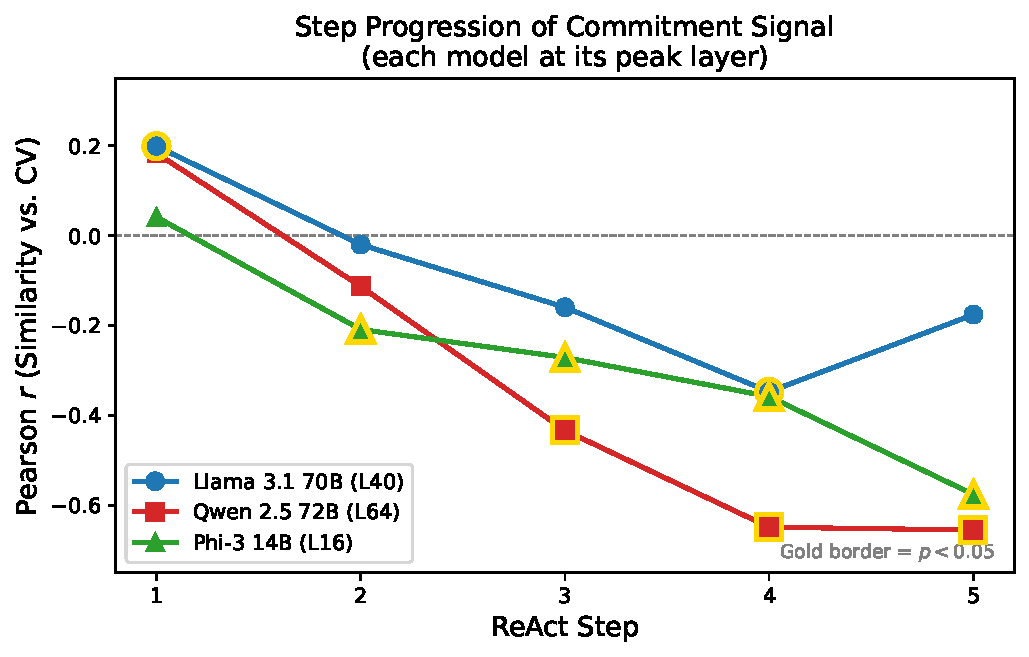
\includegraphics[width=0.8\columnwidth]{figures/multi_model_step_progression.pdf}
\caption{Step progression of the commitment signal across three models (each at its peak layer: Llama L40, Qwen L64, Phi-3 L16). Both 70B models peak at step~4 while Phi-3 (14B) peaks at step~5, suggesting smaller models require one additional evidence-gathering step before committing. Gold borders: $p < 0.05$.}
\label{fig:step_progression_multimodel}
\end{figure}

\section{Commitment Category Visualization}
\label{app:tsne}

Figure~\ref{fig:tsne} shows a t-SNE visualization of step-4 hidden states (layer~40) for all 100 questions, colored by commitment category. Left panel: Llama~3.1~70B; right panel: Qwen~2.5~72B. Hidden states are first reduced to 50 dimensions via PCA, then projected to 2D via t-SNE (perplexity~30). Each point represents one question's mean hidden state across its 10 runs. Committed-correct (green) and committed-wrong (red) questions occupy overlapping regions of the representation space, consistent with our finding that commitment is correctness-agnostic (Section~4.4). Uncommitted-wrong questions (orange) tend toward more diffuse regions, reflecting their higher activation variance.

\begin{figure}[h]
\centering
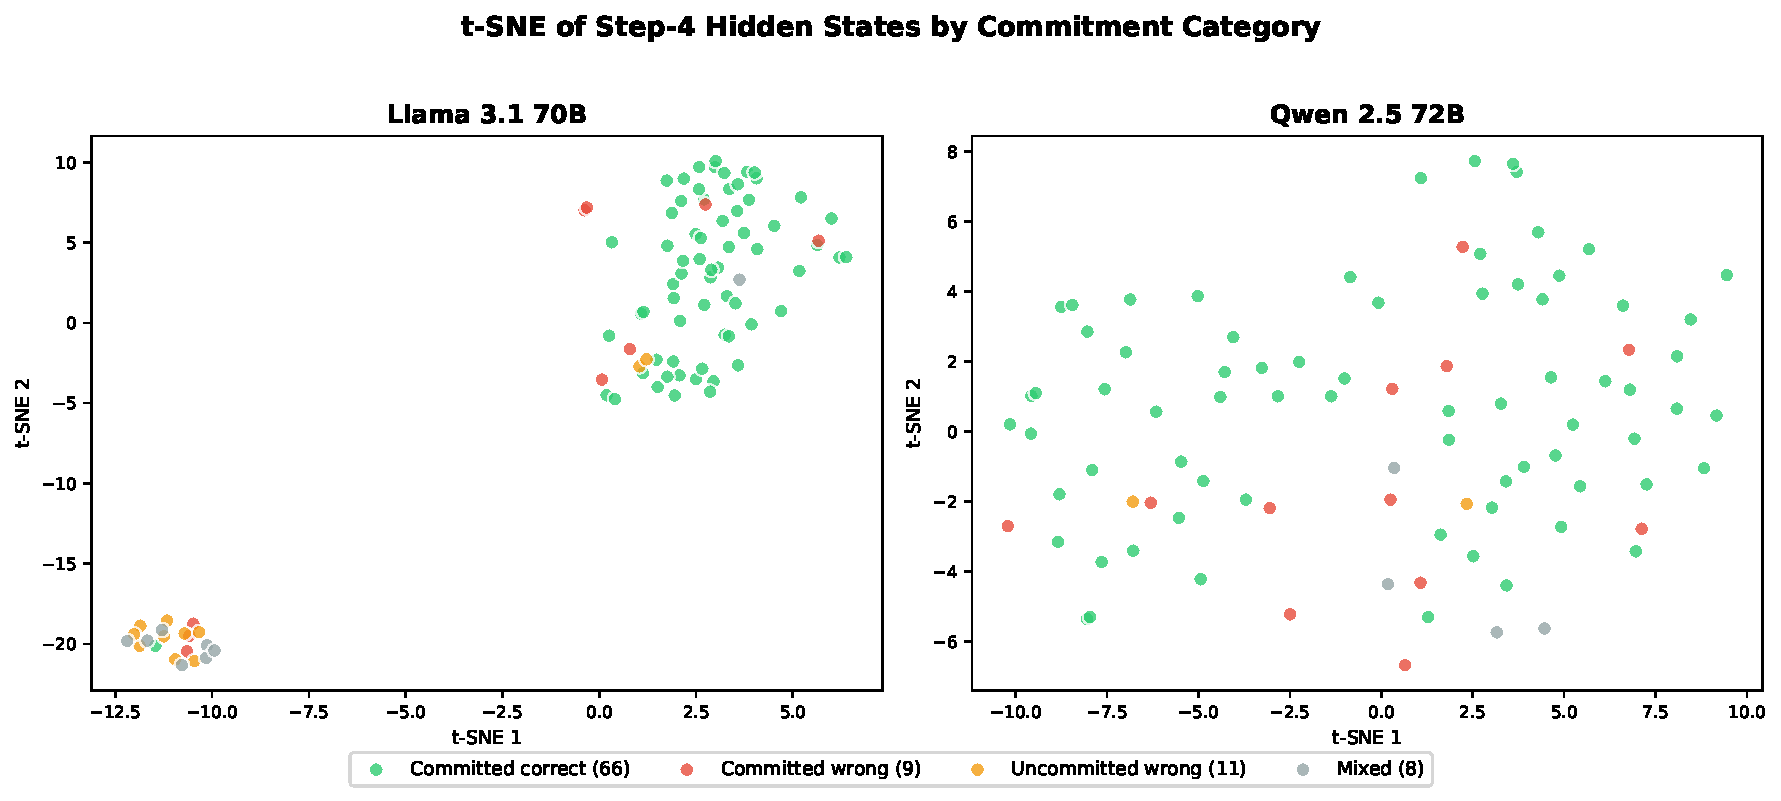
\includegraphics[width=\columnwidth]{figures/commitment_tsne.pdf}
\caption{t-SNE projection of step-4 hidden states (PCA to 50D, then t-SNE to 2D) colored by commitment category. Committed-correct (green) and committed-wrong (red) overlap, confirming that representational commitment is orthogonal to correctness. Uncommitted-wrong (orange) questions show more dispersed representations.}
\label{fig:tsne}
\end{figure}

\section{Baseline Predictors of Behavioral CV}
\label{app:baselines}

Table~\ref{tab:baselines_full} reports the full set of candidate predictors of behavioral CV, including input-level features and downstream behavioral consequences.

\begin{table}[ht]
\caption{Predictors of behavioral CV. $\dagger$Downstream behavioral consequences, not confounds. $\ddagger$Observation overlap measures computed across runs at steps 1--3 ($n = 94$).}
\label{tab:baselines_full}
\centering
\small
\begin{tabular}{lrr}
\toprule
Predictor & $r$ & $p$ \\
\midrule
\textbf{Hidden-state sim.\ (S4, L40)} & $\mathbf{-0.35}$ & $\mathbf{.0006}$ \\
\midrule
TF-IDF obs.\ similarity$^\ddagger$ & $-0.63$ & $< .0001$ \\
Jaccard doc.\ similarity$^\ddagger$ & $-0.40$ & $< .0001$ \\
Search query overlap$^\ddagger$ & $-0.24$ & $.021$ \\
\midrule
Accuracy (correct rate)$^\dagger$ & $-0.31$ & $.002$ \\
Mean total thought length$^\dagger$ & $0.26$ & $.011$ \\
Mean search actions$^\dagger$ & $0.23$ & $.019$ \\
Mean step count$^\dagger$ & $0.21$ & $.037$ \\
\midrule
Question word count & $0.10$ & $.31$ \\
Question char count & $0.12$ & $.25$ \\
N context documents & $0.04$ & $.66$ \\
Mean thought length (S3) & $0.12$ & $.24$ \\
\bottomrule
\end{tabular}
\end{table}

\section{Consistency Prediction: Full Results}
\label{app:runtime}

Table~\ref{tab:runtime_full} reports the complete consistency prediction evaluation across all features, models, and labeling schemes.

\begin{table}[ht]
\caption{Consistency prediction AUROC (95\% CI). Features A--E use step-4 hidden states; baselines use only surface-level input properties.}
\label{tab:runtime_full}
\centering
\small
\begin{tabular}{lcccc}
\toprule
 & \multicolumn{2}{c}{Llama 3.1 70B} & \multicolumn{2}{c}{Qwen 2.5 72B} \\
\cmidrule(lr){2-3} \cmidrule(lr){4-5}
Feature & Quintile & Median & Quintile & Median \\
\midrule
A: Sim (L40) & .93 & .55 & .87 & .86 \\
B: Sim (avg) & .95 & .58 & .90 & .88 \\
C: Layer profile & \textbf{.97} & .73 & .89 & .88 \\
D: Trajectory & .74 & .55 & .77 & .79 \\
E: PCA (L40) & .94 & \textbf{.85} & \textbf{.93} & .67 \\
\midrule
Random & .43 & .57 & .48 & .48 \\
Question length & .52 & .60 & .65 & .57 \\
Context docs & .08 & .06 & .07 & .06 \\
Thought length & .10 & .04 & .00 & .00 \\
\bottomrule
\end{tabular}
\end{table}

\section{StrategyQA Cross-Benchmark Results}
\label{app:strategyqa}

Table~\ref{tab:strategyqa_layers} reports the full layer-wise correlations between activation similarity and behavioral CV at step~3 (the peak step) for Llama-3.1-70B on StrategyQA ($n{=}50$). All layers 8--80 are significant at $p < 10^{-8}$, with partial correlations controlling for accuracy virtually unchanged due to the high overall accuracy (93.2\%).

\begin{table}[ht]
\caption{StrategyQA: Layer-wise correlations at step~3 (Llama-3.1-70B, $n{=}50$). The signal spans all non-embedding layers and peaks at layer~72. Partial correlations control for accuracy.}
\label{tab:strategyqa_layers}
\centering
\small
\begin{tabular}{lcccc}
\toprule
Layer & Raw $r$ & Raw $p$ & Partial $r$ & Partial $p$ \\
\midrule
0  & --- & --- & --- & --- \\
8  & $-0.73$ & $2.5 \times 10^{-9}$ & $-0.72$ & $2.9 \times 10^{-9}$ \\
16 & $-0.78$ & $3.8 \times 10^{-11}$ & $-0.77$ & $4.3 \times 10^{-11}$ \\
24 & $-0.76$ & $2.3 \times 10^{-10}$ & $-0.75$ & $3.7 \times 10^{-10}$ \\
32 & $-0.78$ & $2.6 \times 10^{-11}$ & $-0.78$ & $4.0 \times 10^{-11}$ \\
40 & $-0.81$ & $8.7 \times 10^{-13}$ & $-0.81$ & $8.4 \times 10^{-13}$ \\
48 & $-0.82$ & $2.0 \times 10^{-13}$ & $-0.82$ & $1.9 \times 10^{-13}$ \\
56 & $-0.83$ & $8.8 \times 10^{-14}$ & $-0.83$ & $9.7 \times 10^{-14}$ \\
64 & $-0.83$ & $7.7 \times 10^{-14}$ & $-0.83$ & $9.3 \times 10^{-14}$ \\
\textbf{72} & $\mathbf{-0.83}$ & $\mathbf{7.4 \times 10^{-14}}$ & $\mathbf{-0.83}$ & $\mathbf{9.1 \times 10^{-14}}$ \\
80 & $-0.82$ & $4.8 \times 10^{-13}$ & $-0.82$ & $4.7 \times 10^{-13}$ \\
\bottomrule
\end{tabular}
\end{table}

Table~\ref{tab:crossbenchmark} summarizes cross-benchmark comparison. The StrategyQA signal is stronger than HotpotQA despite a smaller sample, and peaks one step earlier consistent with its shorter reasoning chains.

\begin{table}[ht]
\caption{Cross-benchmark comparison of the representational commitment signal (Llama-3.1-70B). StrategyQA produces a stronger signal that peaks one step earlier, consistent with shorter reasoning chains.}
\label{tab:crossbenchmark}
\centering
\small
\begin{tabular}{lcc}
\toprule
 & HotpotQA & StrategyQA \\
\midrule
Task type & Multi-hop retrieval QA & Implicit reasoning \\
Answer type & Span extraction & Yes/no \\
$n$ (questions) & 100 & 50 \\
Runs per question & 10 & 10 \\
Mean chain length & ${\sim}12$ steps & 5.1 steps \\
Accuracy & 70\% & 93.2\% \\
\midrule
Peak step & 4 & 3 \\
Peak layer & 40 & 72 \\
Peak $r$ & $-0.35$ & $-0.83$ \\
95\% CI & $[-0.48, -0.17]$ & $[-0.90, -0.76]$ \\
Peak $p$ & $< 0.001$ & $< 10^{-13}$ \\
Partial $r$ & $-0.45$ & $-0.83$ \\
Sig.\ layers & 7 / 11 & 10 / 11 \\
\bottomrule
\end{tabular}
\end{table}

Figure~\ref{fig:strategyqa_heatmap} shows the step$\times$layer heatmap of Pearson correlations between activation similarity and behavioral CV for StrategyQA, revealing the sharp commitment signal concentrated at step~3 across all layers.

\begin{figure}[h]
\centering
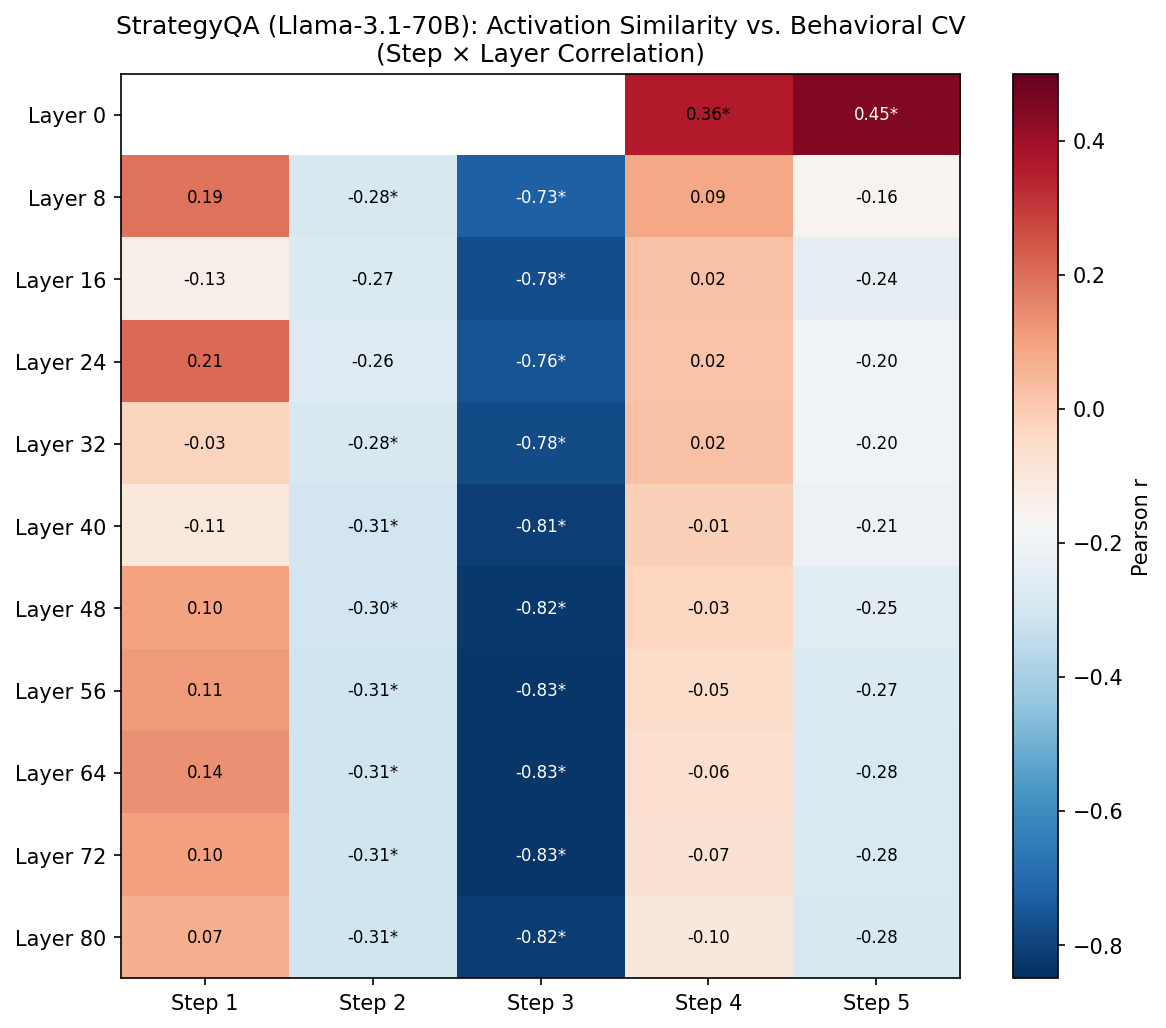
\includegraphics[width=0.7\columnwidth]{figures/strategyqa_heatmap.png}
\caption{StrategyQA step$\times$layer correlation heatmap (Llama-3.1-70B, $n{=}50$). The commitment signal concentrates at step~3 (deep blue column), one step earlier than HotpotQA's step~4 peak, consistent with shorter reasoning chains. All layers 8--80 at step~3 show $|r| > 0.72$ ($p < 10^{-8}$). $^*p < 0.05$.}
\label{fig:strategyqa_heatmap}
\end{figure}

\section{Question-Level Intervention Decomposition}
\label{app:intervention_decomposition}

Figure~\ref{fig:cv_acc_scatter} shows the relationship between CV reduction and accuracy change at the question level under the commitment intervention. Each point is one question; the $x$-axis is $\text{CV}_\text{control} - \text{CV}_\text{commitment}$ (positive = commitment reduced CV) and the $y$-axis is $\text{acc}_\text{commitment} - \text{acc}_\text{control}$ (positive = commitment improved accuracy). The negative correlation ($r = -0.32$, $p = .001$) confirms that commitment amplifies the model's existing trajectory: questions where CV decreased most tended to show slight accuracy decreases, consistent with the correctness-agnostic nature of the commitment signal (Section~4.4).

\begin{figure}[h]
\centering
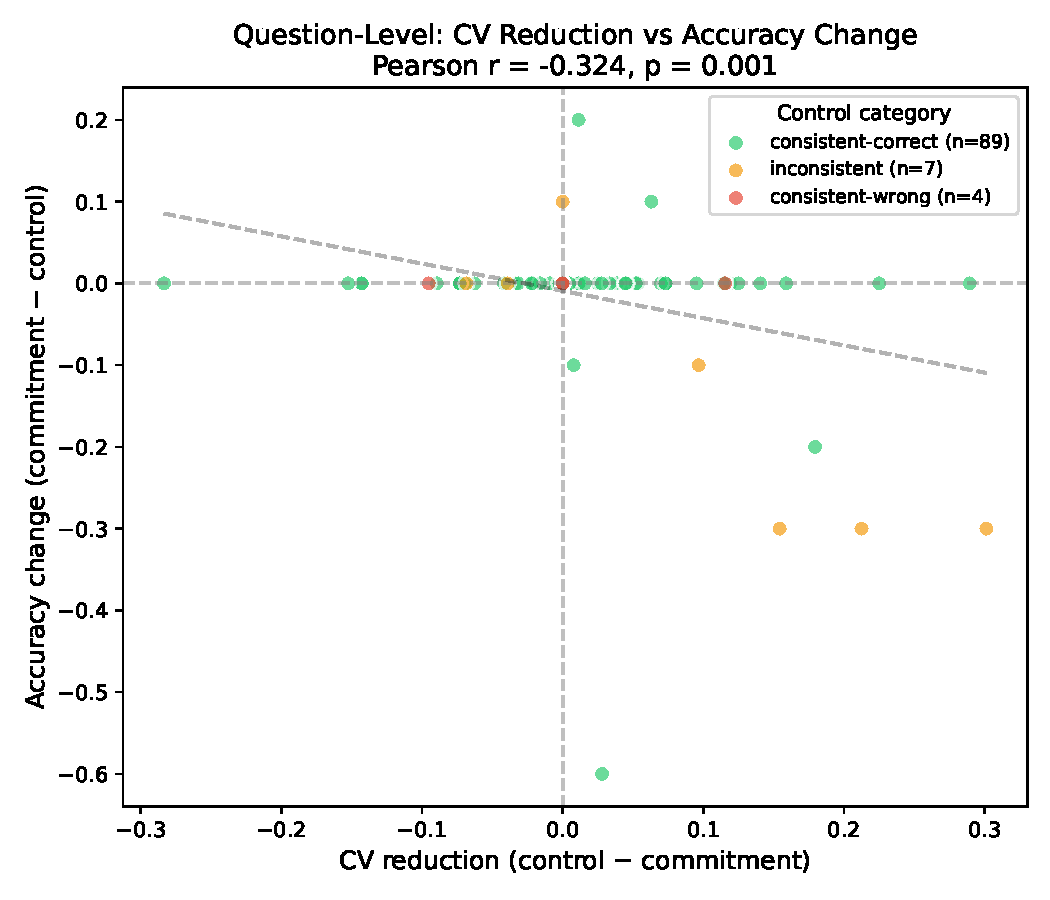
\includegraphics[width=0.7\columnwidth]{figures/task1_cv_acc_scatter.pdf}
\caption{Question-level relationship between CV reduction ($x$) and accuracy change ($y$) under the commitment intervention ($n{=}100$). The negative correlation ($r = -0.32$, $p = .001$) shows that commitment amplifies the model's existing trajectory: lower variance without a systematic accuracy gain.}
\label{fig:cv_acc_scatter}
\end{figure}

\end{document}
